\pagestyle{fancy}
\fancyhead[R]{Física Nuclear y de Partículas: Tema 2}
\fancyhead[L]{4º Grado en Física}
\chapter{Interacciones fundamentales. Leyes de conservación}
\section{Partículas virtuales}
\noindent
\begin{minipage}{0.6\textwidth}
    De manera clásica, cuando introducimos una partícula con carga\footnotemark en el vacío, ésta genera un campo (líneas de campo). Si introducimos otra partícula que tiene el mismo tipo de carga, ésta se verá influida por el campo que ha generado la primera partícula.\\\\
    En mecánica cuántica las interacciones no están mediadas por los campos ``clásicos'' generados por las partículas, sino por partículas denominadas \textbf{bosones gauge} intercambiando momento.
\end{minipage}
\footnotetext{Entendemos carga como la carga asociada a la fuerza.}
\hfill
\begin{minipage}{0.35\textwidth}
    \centering
    \includegraphics[scale=1.2]{Diagramas Tema 2/ParticulaClasica.pdf}
    \captionof{figure}{Campo generado por una partícula clásica.}
    \label{fig: campoclasico}
\end{minipage}\\\\
\noindent \begin{minipage}{0.6\textwidth}
    Si consideramos un electrón siendo influido por una distribución de carga, el bosón gauge del campo electromagnético es el \textbf{fotón}. Vamos a estudiar el scattering desde el sistema CM, para ello nos vamos al vértice del diagrama:
    \begin{itemize}
        \item \textbf{Conservación del momento}:En el vértice pasamos de $e^-(m_ec^2,\vec{0}) \longrightarrow e^-(E_k,-\vec{k}) +
 \gamma(kc,\vec{k})$
        \item \textbf{Conservación de la energía}: En el vértice se conserva la energía $mc^2=\sqrt{m^2c^4+k^2c^2}+kc$, como $\abs{k}\ge 0$ la energía sólo se conserva si $\abs{k}=0$ por lo que, ¿no existe el fotón?
    \end{itemize}
\end{minipage}
\hfill
\begin{minipage}{0.35\textwidth}
    \centering
    \includegraphics[]{Diagramas Tema 2/ElectronDistribcarga.pdf}
    \captionof{figure}{Scattering de un electrón por una distribución de carga.}
    \label{fig: scattering electron y distribucion de carga}
\end{minipage}\\\\
Vamos a hacer de nuevo el análisis pero con partículas masivas. Si tenemos una interacción entre dos partículas $A$ y $B$ de masas $M_A$ y $M_B$ respectivamente que intercambian una partícula masiva $X$ con masa $M_X$ y volvemos realizar el mismo estudio:
\clearpage
\begin{figure}
    \centering
    \includegraphics[width=0.5\linewidth]{Diagramas Tema 2/IntAyB.pdf}
    \caption{Interacción de dos partículas a través de una partícula masiva.}
    \label{fig: intayb}
\end{figure}
\noindent En el primer vértice (línea A) tenemos
    \begin{equation*}
        \begin{aligned}
            &A(M_Ac^2,\vec{0})\longrightarrow A(M_Ac^2,\vec{p})+X(M_Xc^2,-\vec{p})\\ &\Delta E=E_A+E_X-M_Ac^2=\sqrt{M_A^2c^4+p^2c^2}+\sqrt{M_X^2c^4+p^2c^2}-M_Ac^2
        \end{aligned}
    \end{equation*}
Pero antes dijimos que para que se cumpla la conservación de energía la contribución de la energía debía ser nula, por lo que tenemos una \textbf{violación de la conservación energía en el vértice}.\\\\
Esta violación de la conservación de energía \textbf{está permitida} por el principio de incertidumbre, si recordamos
\begin{equation*}
    \Delta E\, \Delta t\sim \hbar \quad  \text{como} \quad E=\sqrt{M^2c^4+p^2c^2}  \Rightarrow \Delta t\sim \frac{\hbar}{\Delta E}
\end{equation*}
Por lo que cuanto mayor sea el incremento de energía, menos tiempo se podrá violar la conservación de energía. Por lo que nos encontramos con dos casos límite
\begin{equation*}
    \Delta E =\left\{\begin{aligned}
    & p \gg M_i \longrightarrow \sqrt{p^2c^2}+\sqrt{p^2c^2}-\cancel{M_Ac^2}=2pc\\
    & p \ll M_i \longrightarrow\sqrt{M_A^2c^4}+\sqrt{M_X^2c^4}-M_Ac^2= M_Xc^2
    \end{aligned} \right.
\end{equation*}
Es concretamente este tipo de partícula lo que conocemos como \textbf{partícula virtual}, es una partícula que no se puede medir ya que su tiempo de vida es tan corto que no podemos medir sus propiedades físicas.\\\\
Entonces como para cualquier valor del momento $\Delta E\ge M_X c^2$  se podrá violar la conservación de energía un tiempo $\tau\sim \dfrac{\hbar}{M_Xc^2}$, ésto nos permite definir una distancia de viaje máxima de las partículas virtuales a través de la expresión $R=c\tau$, que para el caso del fotón como $M_\gamma=0 \Rightarrow \tau= \infty$  y por lo tanto el alcance de dicha interacción es infinito, como ya sabíamos.\\\\
Para el caso de las partículas sin masa como los fotones virtuales \textbf{tampoco se pueden medir} ya que no cumplen la ecuación $E=pc$ ya que se les puede asociar una masa efectiva además de otras características que no tienen los fotones reales.\clearpage
Para otras interacciones tendremos 
\begin{itemize}
    \item \textbf{Interacción débil}: $M_{W^\pm,Z^0}\equiv \unit[80-90]{GeV} \longrightarrow R_\text{Débil}=\unit[2\cdot 10^{-3}]{fm}$, es decir, tienen que estar prácticamente pegadas.
    \item \textbf{Interacción nuclear fuerte}: El alcance que tiene es de $R_\text{fuerte}=\unit[1-2]{fm}$, por lo que la masa de la partícula mediadora debe tener una masa $M\equiv \unit[100-200]{MeV}$. Ésta fue la predicción de Yukawa y en 1947 se descubrió el $\pi^0$ con una masa $M=\equiv \unit[140]{MeV}$.
\end{itemize}
La razón por la que se especifica interacción \textit{nuclear} fuerte, se debe a que es una fuerza residual \footnote{Los quarks tienen color pero sus estados ligados como el protón y el neutrón han de tener color nulo. Sin embargo, cuando están muy cerca los quarks de diferentes nucleones pueden ``verse'' y de ahí nace la fuerza nuclear fuerte.} generada por la interacción fuerte (al igual que las fuerzas de Van der Waals nacen de la interacción electromagnética). La interacción fuerte está mediada por gluones, que son partículas sin masa pero no tiene alcance infinito como la electromagnética, volveremos a este problema más adelante. \label{sec: particulas virtuales}
\section{Intensidad entre interacciones}
\subsection{Potencial de Yukawa}
Si partimos de la ecuación de Klein-Gordon \ref{eq: Ecuacion de Klein-Gordon} para una patícula con masa
\begin{equation}
    -\frac{\hbar^2}{c^2} \pdv[2]{\phi(\vec{r},t)}{t}=-\hbar^2\grad^2\phi(\vec{r},t)+m^2c^2\phi(\vec{r},t)
\end{equation}
obtenemos la ecuación de propagación de un campo bosónico (masivo) arbitrario. Si nuestra función de onda no es función del tiempo, la ecuación resulta la Ecuación de Poisson
\begin{equation}
    \grad^2\phi(\vec{r})=\frac{m^2c^2}{\hbar^2} \phi(\vec{r}) \xrightarrow[\text{Espacio isótropo}]{R=\hbar/mc} \phi(\vec{r})=\phi(r) \Rightarrow \frac{1}{r^2} \pdv{}{r}\qty(r^2\pdv{\phi(r)}{r})=\frac{\phi(r)}{R^2}
\end{equation}
Donde hemos utilizado el laplaciano en esféricas y sólo tenemos contribución de la parte radial por ser el espacio isótropo. Por encontrarnos en esféricas $r>0$ y la solución que encontramos a esta ecuación es 
\begin{equation}
    \phi(r)=\frac{g}{4\pi\,r} \exp{-\dfrac{r}{R}}
    \label{eq: potencial de yukawa}
\end{equation}
Donde $g$ es una constante que nos dará la carga del campo asociado. Para el campo EM la ecuación resultaría la ecuación de Laplace y recuperamos el potencial coulombiano. En el sistema de unidades de Lorentz-Heaviside $(\mu_0=\epsilon_0=1)$
\begin{equation}
    \phi(r)=\frac{g}{4\pi} \frac{1}{e} \Rightarrow V(r)=e \phi(r)=\textcolor{red}{\frac{e^2}{4\pi}}\frac{1}{r} \frac{\hbar c}{\textcolor{red}{\hbar c}}=\textcolor{red}{\alpha} \frac{\hbar c}{r}.
\end{equation}
\clearpage

\subsubsection{Propagadador del potencial de Yukawa}
Si recuperamos el desarrollo que hicimos en el apéndice \ref{chap: Apendice C} la ecuación \ref{eq: transformada de fourier potencial de yukawa} 
$$I_2=\dfrac{4\pi}{\qty(\dfrac{q}{\hbar})^2+\qty(\dfrac{1}{R})^2}$$
es la transformadad de Fourier del potencial de Yukawa salvo la constante de normalización, por lo tanto
\begin{equation}
    A(q)=\frac{g}{4\pi} \dfrac{4\pi}{\qty(\dfrac{q}{\hbar})^2+\qty(\dfrac{1}{R})^2}=g \,\dfrac{\qty(\hbar c)^2}{q^2c^2+M^2c^4}
\end{equation}
Donde hemos vuelto a utilizar que $R=\dfrac{\hbar}{mc}$. Si a la transformada del potencial la multiplicamos por $g$ obtendremos el \textbf{progador}, es equivalente al potencial pero en el espacio de momentos.
\begin{equation}
    f(q)=gA(q)=g^2 \,\dfrac{\qty(\hbar c)^2}{q^2c^2+M^2c^4}
\end{equation}
Podemos definir entonces las constantes de la interacción $g$ como $\alpha_g=\dfrac{g^2}{4\pi \hbar c}$ y el propagador tendrá la forma
\begin{equation}
     f(q)=4\pi \alpha_g\,\dfrac{\qty(\hbar c)^3}{q^2c^2+M^2c^4}
     \label{eq: propagador de yukawa}
\end{equation}
Esta constante $\alpha_g$ nos permitirá saber la intensidad que tiene cualquier interacción. \\\\
A través de la regla de oro de Fermi $\lambda=\dfrac{2\pi}{\hbar} \rho(E) \abs{\mel{f}{V}{i}}^2 \ \text{con} \ \rho(E)=f(\Delta E)$, podemos calcular la  probabilidad de interacción. Como $\lambda\sim \abs{f(q)}^2\sim \alpha_g^2$, la constante de la interacción nos indicará cual es el \textbf{canal más probable para una interacción} (siempre que esté permitido).
\subsubsection{Amplitud de scattering y vértices en los diagramas de Feymann}
Cuando se da una interacción entre partículas, cada una de las partículas tiene un tipo de carga $g$, por lo tanto cuando representamos la interacción en un diagrama de Feymann, cada vértice contribuirá con una cantidad de carga $Z\cdot g$, esto quiere decir que el vértice en el diagrama de Feymann tendrá un valor de $Z\sqrt{\alpha_g}$ ya que recordemos que $\alpha_g\sim g^2$.\\\\
La amplitud de scattering es el elemento de matriz de la regla de oro de Fermi, este elemento va como el producto de cada uno de los vértices del diagrama. Por otro lado la sección eficaz va como el cuadrado del elemento.

\begin{tcolorbox}[colback=airforceblue!20, colframe=airforceblue, title=Ejemplo: Interacción electromagnética]
 En la figura \ref{fig: Interacciones electrones} se represetan dos interacciones permitidas entre electrones, como son de tipo electromagético, la constante de la interacción es la de estructura fina. Las amplitudes y secciones de cada uno de los procesos van como
 \begin{itemize}
     \item Proceso \ref{fig: interaccion electrones sin loop}: \textbf{Amplitud}: $\alpha$ \textbf{Sección eficaz}: $\alpha^2$
     \item Proceso \ref{fig:interaccion loop} \textbf{Amplitud} $\alpha^2$ \textbf{Sección Eficaz}: $\alpha^4$
 \end{itemize}
 Y como la probabilidad de que se de un proceso es proporcional a la sección eficaz, para el caso de la interacción electromagnética $\alpha \sim 10^{-2}$ estos procesos se pueden despreciar frente a otros a la hora de desarrollar una teoría. Pasa lo mismo con las correcciones de estructura fina del átomo de hidrógeno, como las contribuciones a la energía van con $\alpha^2$ se pueden despreciar o tratarse de manera \textbf{perturbativa}
\end{tcolorbox}
\begin{figure}[h!]
    \centering
    % Subfigura 1
    \begin{subfigure}{0.45\textwidth}
        \centering
        \includegraphics[width=0.65\textwidth]{Diagramas Tema 2/IntElectrones.pdf}
        \caption{Interacción electrón-electrón a través de un fotón}
        \label{fig: interaccion electrones sin loop}
    \end{subfigure}
    \hfill
    % Subfigura 2
    \begin{subfigure}{0.45\textwidth}
        \centering
        \includegraphics[width=\textwidth]{Diagramas Tema 2/IntElectronesLoop.pdf}
        \caption{Interacción electrón-electrón a través de un fotón que crea un par electrón-positrón.}
        \label{fig:interaccion loop}
    \end{subfigure}
    
    \caption{Diagramas de Feymann de dos interacciones posibles entre electrones}
    \label{fig: Interacciones electrones}
\end{figure}
\subsection{Constantes de interacciones. Intensidad de las interacciones}
Vamos a calcular las constantes de las interacciones que explicamos al principio del capítulo. Para las dos primeras vamos a considerar un sistema de dos protones separados una distancia $R$\\\\
\noindent
\begin{minipage}{0.4\textwidth}
    \subsubsection{Interacción electromagnética}
El potencial electromagnético se puede escribir como
\begin{equation*}
    V(r)=\frac{e^2}{4\pi \varepsilon_0 } \frac{1}{R} \frac{\hbar c}{\hbar c}= \alpha \frac{\hbar c}{R}
\end{equation*}
El valor de $\alpha\sim 10^{-2}$
\end{minipage}
\hfill
\begin{minipage}{0.5\textwidth}
    \subsubsection{Interacción gravitatoria}
De manera análoga, el potencial gravitatorio va como
\begin{equation*}
    V(r)=- G\frac{m_p^2}{R}\frac{c^4}{c^4} \frac{\hbar c}{\hbar c}=\frac{m_p^2c^4}{\qty(\dfrac{\hbar c}{G})c^4}\frac{\hbar c}{R}=\alpha_\mathrm{G}\frac{\hbar c}{R} 
\end{equation*}
El valor de $\alpha_\mathrm{G}\sim 10^{-39}$
\end{minipage}\\\\
Si calculamos la intensidad relativa entre ambas vemos que el cociente $\alpha_\mathrm{G}/\alpha\sim 10^{-37}$ por lo que nos podemos olvidar de esta interacción en los procesos entre partículas elementales.
\subsubsection{Interacción nuclear fuerte}
Vamos a estudiar dos casos, un sistema ligado y una desintegración:
\begin{itemize}
    \item El primer sistema que vamos a utilizar para calcular esta constante es el \textbf{deuterón} ($p-n$). Lo estudiaremos en su estado fundamental por lo que su energía de ligadura será $B=\unit[-2.225]{MeV}$ y su radio cuadrático medio $\unit[r_\mathrm{D}=1.971]{fm}$. Como las masas de las partículas son mucho mayores que la energía de ligadura, podemos tratar el problema de manera \textbf{no relativista}.\\\\
A través del Teorema del Virial, la energía del sistema la podemos calcular como $E=T+V$. Desarrollando $T$
\begin{equation*}
T=\frac{p^2}{2\mu} \sim \frac{\hbar^2}{R^2 m_p}=\frac{\qty(\hbar c)^2}{m_pc^2R^2}=\unit[2.67]{MeV}
\end{equation*}
Donde hemos utilizado que las masas del neutron y el proón son aproximadamente la misma y que $R=2r_\mathrm{D}$. En virtud del si sustituimos el potencial de Yukawa en el término del potencial, expresado en función de la constante fuerte $\alpha_\mathrm{S}$ obtenemos
\begin{equation*}
    2.67- \alpha_\mathrm{S} \frac{\hbar c}{R} \exp{-\frac{m_\pi c^2}{\hbar c}R}=-2.225 \Rightarrow \alpha_S=\frac{2.67+2.225}{3.376}=1.45 \sim 1
\end{equation*}
\item Vamos a estudiar dos desintegraciones de dos resonancias de la partícula $\Sigma^0$
\begin{equation*}
    \begin{aligned}
        &\Sigma^0(1385) \longrightarrow \Lambda+ \pi^0   \\
        & (2) \quad \Sigma^0(1192) \longrightarrow \Lambda+  \gamma
    \end{aligned}
    \left \} \begin{aligned}
        & \text{Fuerte; $\Gamma=\unit[36.2]{MeV}$, $BR=0.72$}\\
        &\text{EM;  $\tau=\unit[7.4\cdot 10^{-20}]{s}$, $BR=1$}
    \end{aligned} \right.
\end{equation*}
Como son dos procesos de naturaleza distinta podemos calcular el máximo teórico que tienen uno respecto a otro de producirse, para ello volvemos a utilizar la regla de oro de Fermi, en este caso vamos a simplificar las cuentas y a considerar que los espacios fásicos de las dos partículas son aproximadamente iguales, por lo que el cociente irá como $$R=\qty(\dfrac{\alpha_\mathrm{S}}{\alpha})^2=\dfrac{BR_1\cdot\Gamma_1}{\Gamma_2}\sim2900 \Rightarrow \alpha_\mathrm{S}\approx54\alpha \sim 1$$
Del primer proceso, tenemos que el tiempo es de $\tau=\unit[1.82\cdot 10^{-23}]{s}$
\end{itemize}
Como esta constante es del orden de la unidad, \textbf{no} admite teoría de perturbaciones.
\subsubsection{Interacción débil}
Vamos a comparar dos desintegraciones
\begin{equation*}
    \begin{aligned}
        &n\longrightarrow p+e^-+\overline{\nu_e} \\ 
        &\pi^- \longrightarrow e^- + \overline{\nu_e}\\
        &\pi^- \longrightarrow  \mu^- + \overline{\nu_\mu}
    \end{aligned}
\end{equation*}
Si comparamos los tiempo de desintegración tenemos $\tau_n=\unit[885.7]{s}$ y $\tau_\pi=\unit[2.6\cdot 10^{-8}]{s}$
vemos que necesitamos en una nueva escala de tiempos. La presencia del neutrino es lo que nos va a indicar que el proceso es \textbf{débil}.
\newpage
Esta interacción \textbf{necesariamente} tiene que \textbf{conservar la carga} pues el tiempo de vida del electrón es $\tau=\infty$ (es estable). Por otro lado tiene que conservar el número bariónico pues la vida media del proton es de $\tau>\unit[10^{29}]{year}$ (infinitamente superior a la vida del universo).\\\\
Vamos a determinar el orden de magnitud a través de las vidas medias. Vamos a comparar una desintegración del barión $\Lambda^+$, que es un proceso fuerte.
\begin{equation*}
    \Lambda^+\longrightarrow n+\pi^+ \Rightarrow
    \boxed{\Gamma=\unit[114-125]{MeV} \Rightarrow \tau=\unit[5\cdot10^{-24}]{s}}
\end{equation*}
Con la desintegración principal del barión $\Sigma^-$ ($BR=99.8\%$)
\begin{equation*}
    \Sigma^-\longrightarrow n+\pi^- \Rightarrow \boxed{\tau=\unit[1.48\cdot10^{-10}]{s}}
\end{equation*}
Este proceso \textbf{no conserva el sabor}, pues la composición del sigma es $\Sigma^-=dds$, en el estado inicial tenemos $s=-1$ mientras que en el estado final tenemos $s=0$. Si calculamos la razón entre las anchuras como hicimos en la interacción fuerte
\begin{equation*}
    R=\frac{\Gamma(\Lambda^+\xrightarrow{}n+\pi^+)}{\Gamma(\Sigma^-\xrightarrow{}n+\pi^-)}=\qty(\frac{\alpha_\mathrm{S}}{\alpha_\mathrm{W}})^2=\frac{\tau_\Sigma}{\tau_\Lambda}=2.96\cdot 10^{13} \quad \text{como} \quad \alpha_\mathrm{S}\sim 1, \alpha_\mathrm{W}\sim 1.8\cdot 10^{-7}
\end{equation*}
\subsubsection{Comparación de las escalas}
Si conocemos las vidas medias/anchuras de deintegración podemos conocer el proceso. 
\begin{table}[h]
\centering
\begin{tabular}{|c|ccc|}
\hline
Interacción& $\alpha_i$ & $\unit[\tau]{[s]}$ & $[\Gamma]$ \\ \hline
Fuerte           & 1          & $10^{-24}$       & MeV        \\
Electromagnética & $10^{-2}$  & $10^{-20}$       & KeV        \\
Débil            & $10^{-7}$  & $10^{-14} >$      & -          \\
Gravitatoria     & $10^{-39}$ & -                & -         \\ \hline
\end{tabular}
\caption{Tabla comparando las constantes de intensidad, escala de tiempos y rangos de energía. Para el caso de la interacción débil tenemos un rango muy grande.}
\label{tab: comparacion de escalas}
\end{table}
Además siempre que tengamos una desintegración se realizará a través del canal de interacción más rápido (mayor $\alpha_i$) \textbf{cuando esté permitido}.
\subsection{Unificación electrodébil}
De las soluciones estáticas de la ecuacición de Klein-Gordon \ref{eq: Ecuacion de Klein-Gordon} en el espacio de momentos obtenemos el propagador \ref{eq: propagador de yukawa}. Si tenemos bosones mediadores de masa muy grande, nos encontramos en el límite $Mc^2\gg qc$ y así 
\begin{equation}
    f(q)=4\pi \alpha_\mathrm{W} \frac{\qty(\hbar c)^3}{M^2c^4}=G_\mathrm{F}
    \label{eq: constante de Fermi}
\end{equation}
que nos daría la amplitud de la probabilidad de que sucediese un proceso débil. Esta constante se habría medido en núcleo y se denomina \textbf{constante de Fermi} $\dfrac{G_\mathrm{F}}{\qty(\hbar c)^3}=\unit[1.166\cdot 10^{-5}]{GeV^{-2}}$
\clearpage
En 1967/1968, Glashow-Weinberg y Salam, pudieron calcular la masa del bosón mediador de la interacción débil a través de la ecuación \ref{eq: constante de Fermi}
\begin{equation}
    Mc^2=\sqrt{\dfrac{4\pi \alpha_W}{G_\mathrm{F}/\qty(\hbar c)^3}}=\sqrt{\dfrac{4\pi \alpha}{G_\mathrm{F}/\qty(\hbar c)^3}}=\unit[88.7]{GeV}
\end{equation}
Es decir, supusieron que la constante de la interacción débil, no era $\alpha_\mathrm{W}$, sino $\alpha$, la constante de estructura fina, ya que al utilizar la constante débil, la partícula debía tener una masa de $\sim \unit[300]{MeV}$ que coincide con el valor experimental medido posteriormente.\\\\
Por lo tanto la probabilidad de emitir un fotón o un bosón $Z^0,W^\pm$ es la misma en altas energías, a bajas energía como la masa de los bosones débiles son tan descomunales, los procesos débiles son muy poco probables.
\begin{figure}[h!]
    \centering
    % Subfigura 1
    \begin{subfigure}{0.45\textwidth}
        \centering
        \includegraphics[width=0.65\textwidth]{Diagramas Tema 2/ElectronFoton.pdf}
        \caption{Electrón emite un fotón}
        \label{fig: interaccion electrones sin loop}
    \end{subfigure}
    \hfill
    % Subfigura 2
    \begin{subfigure}{0.45\textwidth}
        \centering
        \includegraphics[width=0.65\textwidth]{Diagramas Tema 2/ElectronZ0.pdf}
        \caption{Electrón emite un $Z^0$}
        \label{fig:interaccion loop}
    \end{subfigure}
    
    \caption{Diagramas de Feymann de dos emsiones de un electrón.}
    \label{fig: Emisioones electrones}
\end{figure}

\noindent En el régimen de bajas energías, la primera emisión es proporcional a $q^{-2}$ mientras que la segunda lo es $M^{-2}$, por lo tanto a bajas energías no consideraremos las emisiones de bosones débiles.
\subsection{Universalidad de la interacción débil} 
\begin{minipage}{0.6\textwidth}\label{sec: universalidad de la interaccion debil}
    El electrón es el leptón cargado más ligero y por lo tanto más estable, el muón tiene un factor de ramificación de 1 para la desintegración
    \begin{equation*}
        \mu^-\longrightarrow e^- +\overline{\nu_e}+ \nu_\mu
    \end{equation*}
    Con una vida media $\tau=\unit[2.2\cdot10^{-6}]{s}$. Mientras que la tau tiene dos canales de desintegración de aproximadamente el mismo factor de ramificación 
    \begin{equation*}
        \begin{aligned}
            &\tau^-\longrightarrow e^-+ \overline{\nu_e} +\nu_\tau \Rightarrow BR=0.178\\
        &\tau^-\longrightarrow \mu^- +\overline{\nu_\mu} +\nu_\tau \Rightarrow BR=0.174
        \end{aligned}
    \end{equation*}
Con una vida media $\tau=\unit[2.9\cdot10^{-13}]{s}$.     
\end{minipage}
\hfill
\begin{minipage}{0.35\textwidth}
    \centering
    \includegraphics[width=\textwidth]{Diagramas Tema 2/DesintegracionMuon.pdf}
    \captionof{figure}{Desintegración de un muon en su canal más probable. En el vértice del muón, el bosón $W^-$ es el que se lleva la carga del vértice.}
    \label{fig: desintegracion muon}
\end{minipage}\\\\
El cociente de las masas de los leptones cargados 
    \begin{equation}
        \frac{m_e}{m_\mu}\sim 5\cdot 10^{-3} \quad \frac{m_e}{m_\tau}\sim 3\cdot 10^{-4} \quad \frac{m_\mu}{m_\tau}\sim 6\cdot 10^{-2}
    \end{equation}

Vamos a plantear la siguiente hipótesis: toso los nodos de la interacción débil son iguales y vamos a decir que son iguales que los hadrónicos. Vamos a calcular las anchuras de desintegración anteriores, para ello utilizamos la expresión calculada en el apéndice \ref{chap: Apendice B}, la ecuación \ref{eq: espacio fasico desintegracion a tres cuerpos}; con la regla de oro de Fermi. 
\begin{equation}
    \begin{aligned}
        & \Gamma(\mu^-\longrightarrow e^- +\overline{\nu_e}+ \nu_\mu)=k\qty[\dfrac{G_\mathrm{F}}{\qty(\hbar c)^3}]^2m_\mu^5\\
        &\Gamma(\tau^-\longrightarrow e^-+ \overline{\nu_e} +\nu_\tau)=k\qty[\dfrac{G_\mathrm{F}}{\qty(\hbar c)^3}]^2m_\tau^5\\
        &\Gamma(\tau^-\longrightarrow \mu^-+ \overline{\nu_\mu} +\nu_\tau)=k\qty[\dfrac{G_\mathrm{F}}{\qty(\hbar c)^3}]^2m_\tau^5
    \end{aligned}
\end{equation}
Los factores distintos del espacio fásico están incluidos en la constatante $k$. Si nos fijamos en el diagrama \ref{fig: desintegracion muon} tenemos dos vértices\footnote{Da igual que sea el muón o el tau, es una desintegración a 3 cuerpos de una partícula pesada y dos ligeras.}, de ahí que tengamos un cuadrado en el exponente de la constante de Feymann. Por lo tanto, las anchuras de desintegración de ambos canales del tau han de ser iguales.
\subsubsection{Predicciones}
Si calculamos el valor teórico correspondiente a la desintegración del tau y del muón por el canal electrónico obtenemos.
\begin{equation*}
    \frac{\tau_\tau}{\tau_\mu}=\frac{BR(\tau^-\xrightarrow{} e^-+ \overline{\nu_e} +\nu_\tau)}{BR(\mu^-\xrightarrow{} e^- +\overline{\nu_e}+ \nu_\mu)}\frac{\Gamma(\mu^-\xrightarrow{} e^- +\overline{\nu_e}+ \nu_\mu)}{\Gamma(\tau^-\xrightarrow{} e^-+ \overline{\nu_e} +\nu_\tau)}=\frac{0.178}{1}\frac{m_\mu^5}{m_\tau^5}=1.324\cdot10^{-7}
\end{equation*}
Y si calculamos el experimental
\begin{equation*}
    \frac{\tau_\tau}{\tau_\mu}= \frac{2.903\cdot 10^{-13}}{2.197\cdot 10^{-6}}=1.321\cdot 10^{-7}
\end{equation*}
Como vemos, la teoría coincide con los experimentos. Por lo que podemos concluir que las interacciones del muón (2 familia) y el tau (3 familia) son idénticas con los electrones (1 familia).

\section{Simetrías espacio-temporales y simetrías internas}
Una \textbf{simetría} es una una transformación que deja invariante las ecuaciones del movimiento, esta definición es más general que la invarianza del lagrangiano, que recordemos que puede diferenciarse en una derivada total que \textbf{no dependa} de las velocidades.
\newpage
\subsection{Simetrías espacio-temporales}
Vamos a comparar cómo afectan las simetrías tanto en mecánica clásica como en mecánica cuántica. En mecánica clásica la información de los sistemas viene dada por el lagrangiano $\mathcal{L}=\mathcal{L}(\vec{r_i},\dot{\vec{r_i}};t)$, mientras que en mecánica cuántica la información del sistema está en la función de onda $\Psi(\vec{r},t)$.
\begin{itemize}
\item \textbf{Homogeneidad del espacio}: Si variamos el lagrangiano $\delta \mathcal{L}=0$ obtenemos que \\
$\vec{r_i}\xrightarrow[]{} \vec{r_i}+\vec{a}$ y nos aparece una integral primera del movimiento, el \textbf{momento lineal} $\vec{p}$.\\\\ En mecánica cuántica, si tenemos una función de onda $\Psi_{\alpha^\prime}(\vec{r})=\Psi_{\alpha}(\vec{r}+\vec{a})$, las transformaciones de las funciones de onda sólo pueden hacerlas operadores, para las traslaciones espaciales, tenemos el operador traslación $$\Psi_{\alpha^\prime}(\vec{r})=U(\vec{a})\Psi_{\alpha}(\vec{r})=\exp{-i\frac{\vec{a}\cdot \vec{p}}{\hbar}} \Psi_{\alpha}(\vec{r})$$
La simetría solo se satisface si el operador traslación deja invariante la ecuación de Shcrödinger, y como el operador traslación lo podemos desarrollar en serie de Taylor en potencias del momento, siempre va a conmutar con el hamiltoniano, por lo que el momento se conserva y es el \textbf{generador de las traslaciones espaciales} y forma una estructura de \textbf{grupo}.
    \item \textbf{Homogeneidad del tiempo}: En mecánica clásica si el lagrangiano no depende explícitamente del tiempo (al hacer la traslación temporal no cambia), la cantidad conservada corresponde con el hamiltoniano que cuando no depende del tiempo coincide con la energía.\\\\
    En mecánica cuántica estudiamos los sistemas a través de la ecuación de Schrödinger dependiente del tiempo
    \begin{equation*}
        i\hbar \pdv{\Psi}{t}=H\Psi
    \end{equation*}
    De manera análoga con el operador traslación espacial, el operador traslación temporal tiene la forma $T=\exp{-i\dfrac{H\cdot t}{\hbar}}$ y como el hamiltoniano conmuta consigomismo, el hamiltoniano es el \textbf{generador de las traslaciones temporales}
    \item \textbf{Isotropía del espacio}: Si el espacio es isótropo, el lagrangiano se es invariante bajo rotaciones, por lo que se conserva el \textbf{momento angular} $\vec{L}=$cte.\\\\ En mecánica cuántica no tiene por qué conservarse el momento angular orbital ni el de spin, pero \textbf{siempre} ha de conservarse el \textbf{momento angular total} $\vec{J}=\vec{S}\otimes \vec{L}$
\end{itemize}
\subsection{Internas}
Las simetrías internas son simetrías características de los sistemas que no son función de las coordenadas clásicas. Un ejemplo de simetría interna es el \textbf{isospín}, esta simetría hace indistinguibles al protón y al neutrón frente a una transformación (interacción fuerte).
\newpage
\subsection{Tipos de simetrías}
Las simetrías pueden ser de dos tipos
\begin{itemize}
    \item \textbf{Simetría discreta}: Estas simetrías son multiplicativas por lo tanto si tenemos un conjunto de 
    operadores $P_i$, la simetría total será $$P=\prod_i P_i$$
    \item \textbf{Simetrías contínuas}: Las simetrías continua tienen estructuras de grupo, por lo que son ``aditivas'' en el sentido de la teoría de grupos, un ejemplo es el momento angular $$\vec{L}=\bigoplus_i \vec{\ell_i}$$
\end{itemize}
\section{Paridad}
La paridad tiene una serie de características. Las partículas podemos definirlas en función de su spin y su paridad con la forma $J^P$.
\begin{itemize}
    \item Es una simetría discreta que se caracteriza $\vec{r} \longrightarrow -\vec{r}$. 
    \item Es un obsrevable, por lo tanto es hermítico.
    \item Es un operador unitario, por lo que sus autovalores son $\pm 1$.
    \item Es una simetría de la \textbf{interacción fuerte} y \textbf{electromagnética} pero \textbf{no} de la interacción débil.
\end{itemize}
En función de la paridad podemos clasificar vectores:
\begin{itemize}
    \item \textbf{Vectores polares}: son los vectores que cambian de signo bajo paridad, un ejemplo es el operador traslación y o el operador momento. Se define como $1^-$.
    \item \textbf{Vectores axiales}: son los vectores que no cambian de signo bajo paridad, un ejemplo es el momento angular, ya que $\vec{L}=\vec{r}\times \vec{p}=-\vec{r}\times -\vec{p}=\vec{L} $. Se define como $1^+$.
\end{itemize}
También podemos clasificar escalares:
\begin{itemize}
    \item \textbf{Escalares}: es un escalar de la forma $a=\vec{p_1}\cdot \vec{p_2}\xrightarrow[]{} a$, es decir, es invariante bajo paridad. Definimos su paridad como $0^+$.
     \item \textbf{Pseudoescalares}: es un escalar de la forma $a=\vec{p_1}\cdot \vec{p_2}\xrightarrow[]{} -a$, es decir, no es invariante bajo paridad. Definimos su paridad como $0^-$.
\end{itemize}
Esto nos sirve para clasificar partículas (campos).
\subsubsection{Paridad de un sistema físico. Sistema de dos partículas}
Supongamos que tenemos un sistema de dos partículas que interaccionan a través de un potencial central $    V(\vec{r}=V(r_{12})$, por lo que la función de onda en coordenadas esféricas será $ \Psi_{nml}(\vec{r})=R_{nl}(r)Y_{lm}(\theta,\varphi)$, si hacemos un cambio de paridad $$\vec{r}\xrightarrow[]{} -\vec{r} \Rightarrow \left \{ \begin{aligned}
    &r\xrightarrow[]{} r \\ &\theta \xrightarrow[]{} \pi-\theta\\ &\varphi \xrightarrow[]{} \pi+\varphi
\end{aligned} \right. \xrightarrow[\text{Armónicos esféricos}]{} Y_{lm}(\pi-\theta,\pi+\varphi)=(-)^{l} Y_{lm}(\theta,\varphi)$$
Por lo tanto la paridad sobre la función de onda esféricas actúa $PY_{lm}(\theta,\varphi)=(-)^l Y_{lm} (\theta,\varphi)$.\\\\
Para un sistema de 2 partículas, la simetría bajo intercambio de partículas coincide con la paridad.
\subsubsection{Paridad de un sistema físico. Sistema de $N$ partículas}
Un sistema de \textit{N} partículas está rejido por un potencial $V(\vec{r}_{k=1\dots N})= \displaystyle \sum_{i<j}^N V(\vec{r}_{ij})$ y la función de onda del sistema será el producto de funciones de onda en coordenadas de Jacobi $\Psi(\vec{r}_{k=1\dots N})=\displaystyle \prod^{N-1}_{i=1} \phi(\lambda_i)$, por lo tanto la paridad dela función de onda del sistema será $P\Psi(\vec{r}_{k=1\dots N})=(-)^{L_\lambda}\Psi (\vec{r}_{k=1\dots N})$ con $L_\lambda=\displaystyle {\sum_i^{N-1}l_{\lambda_i}}$\\\\
En un sistema de $N$ partículas sólo tenemos un caso en el que la paridad está determinada de forma \textbf{unívoca}. Cuando tenemos el mismo momento angular relativo ya que la suma de dos enteros iguales siempre es par y podemos tener momento angular total (composición) 0.
\subsection{Paridad Intrínseca}
Si tenemos una partícula libre, su función de onda será $\Psi^a_{\vec{p}} (\vec{x},t)=\exp{-i\dfrac{\vec{p}\cdot \vec{x}-Et}{\hbar}}$ que si aplicamos paridad obtenemos
\begin{equation*}
    \hat{P}\Psi^a_{\vec{p}} (\vec{x},t)= P_a \Psi^a_{\vec{p}} (-\vec{x},t)=P_a \Psi^a_{-\vec{p}} (\vec{x},t)
\end{equation*}
Donde $P_a$ es una fases de módulo 1. Si nos encontramos en reposo $p=0$ y la función es $\Psi^a (\vec{x},t)$ que es autoestado de la paridad y por lo tanto $P_A=\pm 1$.\\\\
Por lo tanto al imponer conservación de paridad en un sistema, tenemos que incluir la paridad intrínseca.
\subsubsection{¿Por qué no ha aparecido en la mecánica cuántica no relativista?}Si recordamos la ecuación de Schrödinger tiene asociada una ecuación de continuidad, esta ecuación conserva el número de partículas, por lo que la paridad se conserva de manera inmediata ya que la paridad de las funciones de onda en el estado final e incial ha de ser la misma.
\subsubsection{¿Cómo se puede determinar la paridad intríseca?}
Este resultado se obtiene de forma natural de la ecuación de Dirac estática, eso no lo vamos a ver por lo que veremos una demostración \textit{ad hoc}.\\\\
Partimos del positronio, este estado ligado se desintegra cuando el momento angular orbital total es 0\footnote{Ya que la contribución del término centrífugo es 0 y no hay divergencia en $r\xrightarrow[]{}0$.}. Sin embargo, tenemos que tener en cuenta el spin, si acoplamos los spines $\dfrac{1}{2} \otimes \dfrac{1}{2}=0\oplus 1$ que corresponden al \textit{para}positronio ($^1S_0$) y \textit{orto}positronio ($^3S_1$) respsectivamente. \\\\
\noindent
\begin{minipage}{0.6\textwidth}
    A tavés de la teoría semiclásica de la radiación podemos estudiar la polarización de los fotones emitidos en la desintegración de un par electrón-positrón. El estado de los fotones viene dado por dos vectores, el vector momento $\vec{k}$ y el vector polarización $\vec{\epsilon}$.\\\\
    Del acoplamiento de los momentos angulares totales obtenemos
    \begin{equation*}
        J_\mathrm{i}=\Vec{L}_{e^-e^+}\otimes \vec{J}_{e^-}\otimes \vec{J}_{e^+}=0\otimes \textcolor{red}{\vec{S}_{e^-}\otimes \vec{S}_{e^+}}=0\otimes \textcolor{red}{0}=0
    \end{equation*}
\end{minipage}
\hfill
\begin{minipage}{0.35\textwidth}
    \centering
    \includegraphics[width=\textwidth]{Diagramas Tema 2/Polarizacionfotones.pdf}
    \captionof{figure}{Esquema de la polarización de dos fotones emitidos por una aniquilación de pares.}
\end{minipage}\\\\

Donde hemos elegido que el acoplamiento del spin sea antisimétrico., como el momento angular inicial es 0, por conservacion del momento también tiene que ser 0 y por lo tanto el fotón es una partícula \textbf{(pseudo)escalar}. Ahora bien, la función de onda la podemos construir a través de 
\begin{equation}
    \begin{aligned}
       & \vec{\epsilon}_1 \cdot \vec{\epsilon}_2 \propto \cos(\varphi) \quad \text{Paridad: } +\\
       &  \qty(\vec{\epsilon}_1 \times \vec{\epsilon}_2 ) \cdot \vec{k} \propto \sin(\varphi)\quad \text{Paridad: } -
    \end{aligned}
    \label{eq: paridad de la polarizacion}
\end{equation}
No podemos utilizar $\vec{\epsilon}_i \cdot \vec{k}=0$, estas cantidades dependen del ángulo de polarización $\varphi=\widehat{\qty(\vec{\epsilon}_1,\vec{\epsilon}_2)}$, por lo tanto el momento angular orbital del estado final $L_{\gamma \gamma}$ tiene que tener la misma polaridad que el término dominante de la función de onda.\\\\
La paridad sí que se conserva en la interacción electromagnética, por ello el estado inicial está bien definido. Con lo cual, vamos a estudiar la paridad:
\begin{itemize}
    \item \textbf{Estado inicial}: La paridad del estado inicial viene dada por la paridad intrínseca de cada uno de los leptones y la paridad del movimiento relativo entre ellos. 
    \item \textbf{Estado final}: La paridad del estado final viene dada por la paridad de cada uno de los fotones y la paridad del momento relativo. Como la paridad intrínseca de los fotones es la misma como vimos al ser un operador unitario, el cuadrado de su valor esperado necesariamente es 1.

\end{itemize}

\begin{equation*}
    \left \{ \begin{aligned}
        &P_\mathrm{i}=P_{e^+}\cdot P_{e^-} \cdot (-)^{L_{e^-e^+}} \\
        &P_\mathrm{f}=P_{\gamma}\cdot P_{\gamma} \cdot (-)^{L_{\gamma \gamma}}=(-)^{L_{\gamma \gamma}}
    \end{aligned} \right. \Rightarrow P_{e^+}\cdot P_{e^-}=(-)^{L_{\gamma \gamma}}
\end{equation*}    

\noindent En 1946 J.A. Wheeler propuso un experimento para determinar la paridad del positrón a través de la aniquilación del par electrón-positrón, con momento angular relativo nulo. Para ello se estudió la polarización de los fotones emitidos en la aniquilación y se observó que la razón entre los fotones cuyas componentes eran perpendiculares y los que cuyas componentes eran paralela era 2, por lo que la contribución dominante era el término proporcional a $\sin(\varphi)$ (antisimétrico) por lo tanto $L_{\gamma \gamma}=$impar. Por lo tanto el positrionio es un \textbf{pseudoescalar} $0^-$
\subsection{Convenio de paridad en partículas y antipartículas}
Como acabamos de ver, el positronio es una partícula pseudoescalar, podemos decir que la paridad intrínseca de las partículas y las antipartículas está relacionada por
\begin{equation}
    P_f\cdot P_{\Bar{f}}=-1
\end{equation}
Así la paridad de la partículas será positiva y la de las antipartículas será negativa. Cabe mencionar que la paridad satisface el teorema de spin-estadística, así podemos determinar la razón entre la paridad de un mesón y un antimesón es
\begin{equation}
    \left.\begin{aligned}
        &P_M=P_q\cdot P_{\Bar{q}} (-)^{L_{q\Bar{q}}}=(-)^{1+L_{q\Bar{q}}} \\
        &P_{\Bar{M}}=P_q\cdot P_{\Bar{q}} (-)^{L_{q\Bar{q}}}=(-)^{1+L_{q\Bar{q}}}
    \end{aligned} \right \} \Rightarrow P_M \cdot P_{\Bar{M}}=1
\end{equation}
Con lo que obtenemos cómo se relacionan la paridad intrínseca de los \textbf{bosones}.\\\\
De manera análoga podemos obtener la paridad de los bariones
\begin{equation}
        \left.\begin{aligned}
        &P_B=P_{q_1}\cdot P_{q_2} \cdot P_{q_3} (-)^{L_{12}} (-)^{L_{(12)3}} \\
        &P_{\Bar{B}}=P_{\Bar{q_1}}\cdot P_{\Bar{q_2}} \cdot P_{\Bar{q_3}} (-)^{L_{12}} (-)^{L_{(12)3}}
    \end{aligned} \right \} \Rightarrow P_B \cdot P_{\Bar{B}}=-1
\end{equation}
\subsubsection{Paridad del fotón}
Partimos de la ley de Gauss para el campo eléctrico.
\begin{equation}
\div \vec{E}(\vec{r},t)=\frac{1}{\varepsilon_0} \rho(\vec{r},t)
\label{eq: ley de gauss}
\end{equation}

Para que esta ecuación del movimiento sea invariante bajo paridad, tenemos que cambiar$$\vec{r}\xrightarrow[]{}-\vec{r}, \quad \grad \xrightarrow[]{} -\grad, \quad \rho(\vec{r},t) \xrightarrow[]{} \rho(-\vec{r},t), \quad \vec{E}(\vec{r},t) \xrightarrow[]{} -\vec{E}(-\vec{r},t)$$
Si suponemos que estamos en el vacío, $\vec{J},\rho=0$.
El campo eléctrico lo podemos expresar en función del potencial de eléctrico y el potencial vector a través del teorema de Helmholtz
\begin{equation}
    \vec{E}(\vec{r},t)=-\grad \phi -\frac{1}{c} \pdv{\vec{A}(\vec{r},t)}{t}
    \label{eq: campo electrico y potenciales}
\end{equation}

Si fijamos del gauge de Coulomb $\displaystyle \left \{ \begin{aligned}
&\phi(\vec{r},t)=0\\
& \div \vec{A}(\vec{r},t)=0
\end{aligned}\right.$ el campo eléctrico sólo depende del potencial vector y como hemos visto, el campo eléctrico tiene paridad $\vec{E}(\vec{r},t) \xrightarrow[]{} -\vec{E}(-\vec{r},t)$, por lo que el potencial vector ha de tener la misma $\vec{A}(\vec{r},t) \xrightarrow[]{} -\vec{A}(-\vec{r},t)$, como el fotón tiene spin 1 es una \textbf{partícula vectorial polar}, $1^-$.

\subsubsection{Determinación experimental de la paridad del pión}

Como sabemos el pión es el mesón más ligero $\sim \unit[140]{MeV}$, en el estado más ligero que puede tener (onda S), el momento angular orbital relativo es 0 (par)\footnote{Esto aplicará tanto para bariones como mesones.}, por lo tanto para el pión $\pi^-=d\overline{u}$, el momento angular total $\vec{J}=\vec{L}\otimes \vec{S}=0$ y al igual que el positronio es una partícula \textbf{pseudoescalar}.\\\\
La paridad del pión se midió mucho antes de postular los quarks, a través de la absorción\footnote{Un proceso de absorción implica que \textbf{no} tenemos que aportar energía para vencer la barrera centrífuga de la ecuación de Schrödinger de un potencial central, por lo que \textbf{sólo se da en estados de onda S}.} de piones por el deuterón.
\begin{equation}
    \pi^- +d \longrightarrow n+n
\end{equation}
El deuterón es un estado ligado de un protón y un neutrón, esta partícula es un bosón por lo tanto si acoplamos los spines obtenemos $S=1$ \footnote{Los spines de una partícula con estructura son la composición de todos los momentos angulares que forman el sistema.} , mientras que el momento angular orbital toma valores $L=0,2$; que escogiendo el estado de onda S, podemos acoplar los momentos angulares obteniendo $J=L\otimes S=0\otimes 1=1$.\\\\
La paridad del sistema será 
\begin{equation*}
    P_{\pi^-} \cdot P_d (-)^{L_{\pi^- d}}=(P_n)^2 (-)^{L_{nn}} \Rightarrow P_{\pi^-} =(-)^{L_{nn}}
\end{equation*}
Donde hemos utilizado que la paridad del deutrón y la del neutrón es positiva y que $L_{\pi^-d}=0$. Por otro lado en el estado final la función de onda es completamente antisimétrica y la podemos descomponer en dos partes, una radial y otra correspondiente al momento angular total $\Psi_{nn}=\psi_{nn}(r)\chi_{nn}$. La paridad de la función de momento angular total nos la dará el momento angular total, por ello utilizamos la conservación del momento angular total en el sistema.
\begin{equation}
    \begin{aligned}
        & \vec{J}_\mathrm{i}= \vec{J}_{\pi^-} \otimes \vec{J}_d \otimes \vec{L}_{\pi^-d}=0\otimes 1 \otimes \Rightarrow  \vec{J}_\mathrm{i}=1 \\
        & \vec{J}_\mathrm{f}= \vec{J}_n \otimes \vec{J}_n \otimes \vec{L}_{nn}=\frac{1}{2}  \otimes  \frac{1}{2} \otimes  L_{nn}
    \end{aligned}
\end{equation}
\clearpage
Al acoplar $\dfrac{1}{2} \otimes \dfrac{1}{2}=0\oplus 1$ vemos dos situaciones \label{sec: estado ligado de dos neutrones}
\begin{itemize}
    \item 0: Esta función de spin es \textbf{antisimétrica} por lo que la función radial tiene que ser simétrica y por lo tanto el momento angular orbital relativo $L_{nn}$ tiene que ser par, que al acoplarlo con 0 nos da un momento par, que viola el pcpo de exclusión de Pauli.
    \item 1: Esta función de spin es \textbf{simétrica} por lo que la función radial tiene que ser antisimétrica y el momento angular orbital relativo $L_{nn}$ tiene que ser impar, que al acoplarlo con 1 nos da un momento impar, de hecho, el único momento que al acoplarlo con 1 nos da 1 es 1 por lo que $L_{nn}=1$ (onda P).
\end{itemize}
Con lo que hemos demostrado que el pion es una partícula pseudoescalar. Si el pión tuviese paridad positiva esta reacción no se debería observar a través de la interacción fuerte.\\\\
Por último nos falta mencionar que los \textbf{neutrinos no tienen paridad definida} pues la interacción débil no conserva la paridad.
\subsection{Paridad C}
\begin{itemize}
    \item Es una simetría discreta que se caracteriza por camibar $\text{Partícula} \longleftrightarrow \text{Antipartícula}$ sin modificar grados de libertad espaciales o internos. 
    \item Es un obsrevable, por lo tanto es hermítico.
    \item Es un operador unitario, por lo que sus autovalores son $\pm 1$.
    \item Es una simetría de la \textbf{interacción fuerte} y \textbf{electromagnética} pero \textbf{no} de la interacción débil.
\end{itemize}
Como la paridad C cambia partículas por antipartículas, cambia todas las ``cargas'' conocidas: $Q,B,L,\Tilde{S}\dots$ 
\begin{equation}
    C QC^\dagger=-Q \hspace{1cm}
       C L_iC^\dagger=-L_i \hspace{1cm}
       C BC^\dagger=-B \hspace{1cm} C\Tilde{S}C^\dagger=-\Tilde{S}
\end{equation}
Vamos a ver cómo se comporta el operador conjugación de carga frente a los autoestados de los operadores de carga. Si tenemos un autoestado del operador $Q$, tenemos $Q\ket{a}=q_a\ket{a}$, pero qué sucede si aplicamos C-paridad antes ó después de aplicar $Q$:
$QC\ket{a}=Q\ket{\overline{a}}=q_{\overline{a}}\ket{\overline{a}}$, pero si aplicamos $CQ\ket{a}=C q_a\ket{a}=q_aC\ket{a}=q_{a}\ket{\overline{a}}$. Como vemos los estados con carga no son autoestados del operador paridad pero, esto nos hace ver que sí que existen autoestados del operador paridad, son aquellos autoestados cuyas cargas sean todas 0, como es el caso del fotón o del $\pi^0$.
\subsubsection{Paridad C del ${\pi^0}$}
En la naturaleza observamos que los piones neutros se desintegran en dos fotones 
\begin{equation*}
    \pi^0\longrightarrow \gamma+\gamma \xrightarrow[\text{C-Paridad}]{} C_{\pi^0}=\qty (C_\gamma)^2=+1\Rightarrow J^{PC}(\pi^0)\equiv 0^{-+}
\end{equation*}
Donde hemos utilizado que la C-Paridad es  una simetría discreta, por lo que la ley de conservación es multiplicativa.
\subsubsection{Paridad C del fotón}
Hagamos lo mismo que para determinar la paridad intrínseca del fotón. A partir de la ecuación \ref{eq: campo electrico y potenciales}, como el potencial vector cambia de signo al cambiar de signo del campo eléctrico, por lo que la paridad C del fotón es $C_\gamma=-$ y lo podemos representar como $J^{PC}(\gamma)=1^{--}$

\begin{tcolorbox}[colback=airforceblue!20, colframe=airforceblue, title=Ejemplo: Desintegracion del pion neutro en 2 y 3 fotones]
 Como hemos visto la C paridad del fotón es $C_\gamma=-1$ mientras que la del $\pi^0$ $C_{\pi^0}=+1$. Supongamos que tenemos los siguientes procesos electromagnéticos
 \begin{equation*}
     \pi^0\longrightarrow \gamma+\gamma \hspace{2cm} \pi^0\longrightarrow \gamma+\gamma+\gamma
 \end{equation*}
 Si comparamos las anchuras de desintegración, el espacio fásico de ambas reacciones es el mismo, pero no lo será el elemento de matriz, por lo que la razón entre las anchuras dependerá de la constante de estructura fina
 \begin{equation*}
     R_\mathrm{Th}=\frac{\Gamma(\pi^0\xrightarrow[]{} \gamma+\gamma+\gamma)}{\Gamma(\pi^0\xrightarrow[]{} \gamma+\gamma)}=\frac{\alpha^3}{\alpha^2}\sim 10^{-2}
 \end{equation*}
 Sin embargo experimentalmente se ha comprobado que $R\ll 3\cdot 10 ^{-8}\ll\alpha$ \footnotemark, es decir, que el proceso $\pi^0\xrightarrow[]{} \gamma+\gamma$ es un \textbf{proceso prohibido}. La razón por la que está prohibido se debe a que no conserva la C-paridad ya que en el estado inicial la C-paridad es 1 mientras que en el final es $-1=C_\gamma \cdot C_\gamma \cdot C_\gamma$.
\end{tcolorbox}
\footnotetext{Podríamos pensar que el proceso no es electromagnético, sino que es débil, pero debido a la presencia de los fotones es imposible que lo sea.}

\noindent Tenemos más partículas que tienen paridad C bien definida. 
\begin{equation*}
    \begin{aligned}
        &\rho_0\longrightarrow \pi^0+\gamma \Rightarrow C_{\rho_0}=- \\
        & \eta \longrightarrow \gamma+\gamma \Rightarrow C_{\eta}=+\\
        &\omega \longrightarrow \pi^0 +\gamma \Rightarrow C_{\omega}=-
    \end{aligned}
\end{equation*}
\subsubsection{Paridad C de sistemas partícula-antipartícula}
Como hemos mencionado antes, la paridad C no afecta a los grados de libertad espaciales ni internos. Supongamos que tenemos un fermión y un antifermión en un estado ligado, la función de onda del sistema es
\begin{equation}
    \Psi(1,2)=\frac{1}{\sqrt{2}} \qty[\textcolor{blue}{\psi_f (1)\psi_{\bar{f}} (2) }\textcolor{red}{\phi_L(\vec{r}_{12}) \chi_S(\xi_1,\xi_2)}-\textcolor{blue}{\psi_f (2)\psi_{\bar{f}} (1)}\textcolor{red}{ \phi_L(\vec{r}_{21}) \chi_S(\xi_2,\xi_1)}]
\end{equation}
Si aplicamos C-paridad a la parte \textcolor{blue}{fermiónica} de la función de onda vemos que $C\psi_f (1)\psi_{\bar{f}} (2)= \psi_f (2)\psi_{\bar{f}} (1)$, es decir, al aplicar C-paridad hemos cambiado la partícula 1 por la partícula 2. \\\\
La parte \textcolor{red}{espacial y de spin} bajo intercambio de partículas se ven afectadas
\begin{equation*}
    \begin{aligned}
        &\phi_L(\vec{r}_{12})=(-)^L \phi_L(\vec{r}_{21}) \quad \text{Debido al armonico esferico} \\
        & \chi_S(\xi_1,\xi_2)= (-)^{S-s_1-s_2} \chi_S(\xi_2,\xi_1)
    \end{aligned}
\end{equation*}
Por lo tanto si aplicamos la C-paridad a la función de onda de un par partícula-antipartícula $$C\Psi(1,2)=-(-)^L(-)^{S-2s_f}\Psi(1,2)=(-)^{L+S}$$
El primer menos sale de que la función tiene que ser completamente antisimétrica, y hemos utilizado que la partícula y la antipartícula tienen el mismo spin y por ser fermiones al ser semientero, su contribución y la de la antisimetría de la función hace que se cancelen $-(-)^{2s_f=\text{impar}}=+1$ \footnote{Recordar que $S=s_f \otimes s_{\bar{f}}$ y $L=\ell_1 \otimes \ell_2$.}. Por lo tanto, tenemos que 
\begin{equation}
    C\Psi(1,2)=(-)^{L+S} \Psi(1,2)
\end{equation}
Para el caso de los bosones la función de onda es completamente simétrica
\begin{equation}
    \Psi(1,2) = \frac{1}{\sqrt{2}} \qty[\psi_f (1)\psi_{\bar{f}} (2) \phi_L(\vec{r}_{12}) \chi_S(\xi_1,\xi_2) + \psi_f (2)\psi_{\bar{f}} (1) \phi_L(\vec{r}_{21}) \chi_S(\xi_2,\xi_1)]
\end{equation}

\noindent Al aplicar la C-paridad tenemos $$C\Psi(1,2)=+(-)^{L}(-)^{S-2s_b}\Psi(1,2)$$ en este caso el spin de los bosones $s_b$ es un entero, por lo que la contribución es par y concluimos
\begin{equation}
    C\Psi(1,2)=(-)^{L+S} \Psi(1,2)
\end{equation}
De manera análoga al ejemplo del $\pi^0$, si estudiamos la desintegración del positronio en el estado $^1S_0$, no podemos generar 3 fotones ya que viola la paridad C, el resultado al comparar las anchuras de desintegración teóricas y las experimentales es que $R_\mathrm{th}\sim \alpha \sim 10^{-2}; R_\mathrm{exp}<10^{-5}$.
\section{Isospín}
\noindent
\begin{minipage}{0.6\textwidth}
    El isospín es una simetría de la interacción fuerte. El isospin nace al estudiar lo que se conocen como \textbf{núcleos espejo}, estos núcleos tienen el mismo número de nucleones $A$, estos núcleos tienen un nivel energético muy parecido, es decir, a primer orden podríamos considerarlos \textbf{iguales}.\\\\ Un ejemplo está en la figura \ref{fig: niveles de energia A7}, como vemos hay una pequeña diferencia entre los niveles de energía entre los núcleos del litio y el berilio y eso se debe a correcciones electromagnéticas.
\end{minipage}
\hfill
\begin{minipage}{0.35\textwidth}
    \flushright
    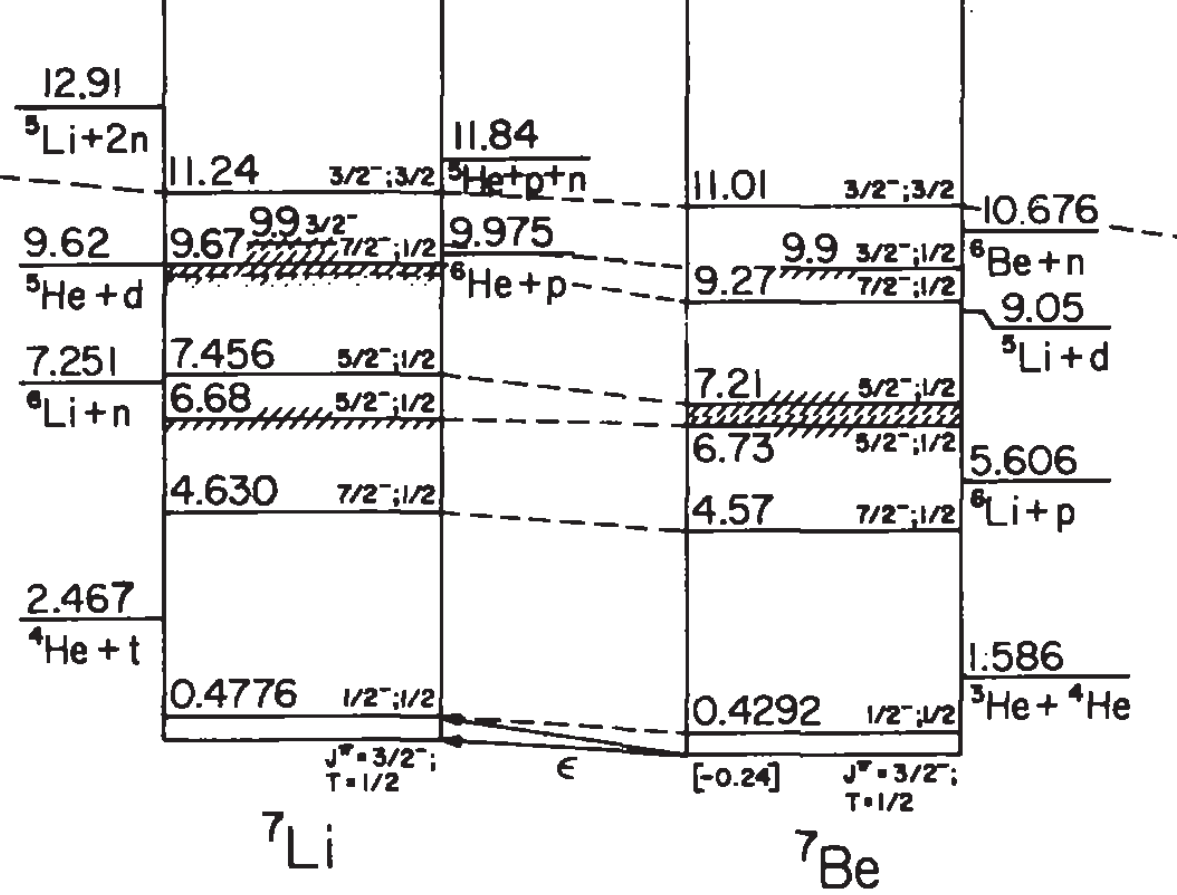
\includegraphics[width=\linewidth]{Imagenes/NivelesEnergiaA7.png}
     \captionof{figure}{Niveles de energía de núcleos con $A=7$.}
     \label{fig: niveles de energia A7}
\end{minipage}
\newpage
\noindent
\begin{minipage}{0.6\textwidth}
    Un ejemplo más ilustrativo son los núcleos con $A=6$ concretamente en $^6\text{He},^6\text{Li},^6\text{Be}$ podemos describir los núcleos como (p,n), por lo tanto tenemos $^6\text{He}=(2,2)+(0,2),^6\text{Li}=(2,2)+(1,1),^6\text{Be}=(2,2)+(2,0)$. Como vemos hay una simetría entre el $^6\text{He}$ y $^6\text{Be}$ ya que hemos cambiado los neutrones por protones respectivamente.
\end{minipage}
\hfill
\begin{minipage}{0.35\textwidth}
    \centering
\begin{tabular}{|ccc|}
\hline
Núcleo        & p & n \\
\hline \hline
$^6\text{He}$ & 2 & 4 \\
$^6\text{Li}$ & 3 & 3 \\
$^6\text{Be}$ & 4 & 2 \\
\hline
\end{tabular}
\captionof{table}{Nucleones dentro de los núcleos con $A=6$.}
\label{tab: Nucleos A6}
\end{minipage}
\\\\ Como la energía de los núcleos es más o menos la misma, la simetría de isospín es \textbf{independiente de la carga}, además la existencia de un estado intermedio como es el $^6\text{Li}$ tenemos que al cambiar protones por neutrones, lo hacemos \textbf{nucleón a nucleón} y no varios a la vez.
\subsection{Analogía de Heisenberg. El espacio de isospín}
En los experimentos de Stern-Gerlach (1922), se observo que en presencia de un campo magnético el electrón se definía en 2 estados y como $2s_e+1=2 \Rightarrow s_e=1/2$. Estos estados correspondían con las proyecciones del spin, $\ket{1/2,1/2},\ket{1/2,-1/2}$.
\\\\
Si recordamos la tabla \ref{tab: Bariones} el neutrón y el protón tienen masas prácticamente iguales y los experimentos nos dicen que ambos tienen la misma $J^p\equiv 1/2^+$, pero hay una pequeña diferencia, y es que mientras que el protón es estable $\tau=\infty$ el neutrón no lo es $\tau=\unit[885.7]{s}$, que se desintegra por el canal débil. Debido a que los núcleos espejos tienen propiedades muy similares, la única interacción que nos queda para explicar esta simetría debe ser la \textbf{interacción fuerte}\footnote{No puede ser débil ya que el neutrón se desintegra y queremos cambiar protones por neutrones y por EM tampoco ya que el neutrón no tiene carga eléctrica.}. \\\\
El neutrón se descubrió en 1932 y en ese mismo año Heisenberg postuló que el protón y el neutrón no eran más que dos posibles estados de una partícula que denominó \textbf{nucleón}. Como había sólo dos posibles estados definió un nuevo número cuántico llamado \textbf{isospín}\footnote{\textit{Spín} de los \textit{isó}topos, spin isotópico.} por lo tanto podemos definir los estados
\begin{equation*}
    2I_N+1=2 \Rightarrow I_N=1/2 \left \{ \begin{aligned}
        &\ket{I\,I_3}=\ket{1/2 , 1/2}\equiv \ket{p}\\
        &\ket{I\,I_3}=\ket{1/2 , -1/2}\equiv \ket{n}
    \end{aligned} \right.
\end{equation*}
Podemos entonces calcular la carga, en unidades de $e$, de los bariones mediante el isospín a través de $Q=I_3+1/2$. Además por ser dos estados de la misma partícula para la interacción fuerte los nucleones tienen la \textbf{misma masa} y son \textbf{indistinguibles} para esta interacción.
\subsubsection{Espacio de isospín}
El isospín se tiene las mismas propiedades que un operador tipo momento angular, por lo tanto el conmutador de sus componentes debe ser $[I_i,I_j]=i\hbar \epsilon_{ijk}I_k$ y como $I^2=\sum^3_i I_i^2$ debe conmutar $[I^2,I_i]=0$, por lo tanto podemos construir los estados igual que en el caso del spin y el momento angular una base que diagonalice en $\qty{I^2,I_3}$.\\\\
Por ser un operador tipo momento angular, los autovalores de los estados propios $\ket{I,I_3}$ son $I^2\ket{I,I_3}=\hbar^2I(I+1)\ket{I,I_3}$ y $I_3\ket{I,I_3}=\hbar I_3\ket{I,I_3}$.\\\\
Supongamos que, al igual que el momento angular total es conservado por el Hamiltoniano de Schrödinger, el isospín lo será para la interacción fuerte, $\qty[H_\mathrm{S},\vec{I}]=0$ y calculamos el elemento de matriz $\mel{I^\prime, I_3^\prime}{H_\mathrm{S}}{I,I_3}$:
\begin{itemize}
    \item Dependencia en la tercera componente $\mel{I, I_3^\prime}{H_\mathrm{S}}{I, I_3}$ $$0=\mel{I, I_3^\prime}{\qty[H_\mathrm{S},I_3]}{I, I_3}=\hbar(I^\prime_3-I_3)\mel{I, I_3^\prime}{H_\mathrm{S}}{I, I_3}\sim \delta_{I_3^\prime I_3}$$
    
    \item Dependencia en el isospín total $\mel{I^\prime, I_3}{H_\mathrm{S}}{I, I_3}$ $$0=\mel{I^\prime, I_3}{\qty[H_\mathrm{S},I^2]}{I, I_3}=\hbar^2(I^\prime (I^\prime+1)-I(I+1))\mel{I^\prime, I_3}{H_\mathrm{S}}{I, I_3}=\hbar^2(I^\prime-I)(I^\prime+I+1)$$ Como el término $I^\prime+I+1$ nunca puede ser 0 necesariamente $I^\prime=I$ por lo tanto $\mel{I^\prime, I_3}{H_\mathrm{S}}{I, I_3}\sim \delta_{I^\prime I}$.

    \item El autovalor del hamiltoniano de la interacción fuerte depende únicamente del isospín total y no sólo de la tercera componente $\mel{I^\prime, I_3^\prime}{H_\mathrm{S}}{I, I_3}$: 
    Como $\qty[H_\mathrm{S}, \vec{I}]=0$ también lo harán los operadores escalera del isospín $\qty[H_\mathrm{S},I_\pm]$, recordamos que al aplicar un operador escalera sobre un estado $I_\pm\ket{I,I_3}=\hbar\sqrt{I(I+1)-I_3(I_3\pm 1)} \ket{I,I_3\pm1}$, por lo tanto $$0=\mel{I,I_ 3}{\qty[H_\mathrm{S},I_+]}{I, I_3-1}\Rightarrow \mel{I,I_3}{H_\mathrm{S}I_+}{I, I_3-1}=\mel{I,I_3}{I_+H_\mathrm{S}}{I, I_3-1}$$ $$\hbar\sqrt{I(I+1)-I_3(I_3- 1)}\mel{I^\prime, I_3^\prime}{H_\mathrm{S}}{I, I_3}=\hbar\sqrt{I(I+1)-I_3(I_3- 1)} \mel{I^\prime, I_3^\prime-1}{H_\mathrm{S}}{I, I_3-1}$$
    $$\mel{I^\prime, I_3^\prime}{H_\mathrm{S}}{I, I_3}=\mel{I^\prime, I_3^\prime-1}{H_\mathrm{S}}{I, I_3-1}$$
    Por lo tanto el elemento de matriz no puede depender de la tercera componente, sólo del isospín total, $\mel{I,I_3}{H_\mathrm{S}}{I,I_3}=A_I $.
\end{itemize}
En conclusión, la interacción fuerte no depende de la tercera componente de isospín, aunque si del isospín total. 
\begin{equation}
    \mel{I^\prime, I_3^\prime}{H_\mathrm{S}}{I,I_3}=A_I\delta_{I^\prime I}\delta_{I_3^\prime I_3}
    \label{eq: elemento de matriz del hamiltoniano fuerte}
\end{equation}
Es decir, una vez especificiado el isospín total, no se distingue entre el protón y el neutrón. Así, calculamos los estados de dos partículas en el espacio de isospín total.

\subsection{Interacción Nucleón-Nucleón. Teorema de Spin-Estadísitca}
Vamos a estudiar cómo interaccionan dos nucleones, para ello conocemos que el isospín total del protón y del neutrón es el mismo $I_1¡=I_2=1/2$ si acoplamos este spin tenemos $\dfrac{1}{2}\otimes \dfrac{1}{2}=0\oplus 1$. Los estados que con acoplamiento a $I=1$
\begin{equation}
\begin{aligned}
    &\ket{11}=\ket{1/2,1/2} \otimes \ket{1/2,1/2} \equiv \ket{pp}\quad \ \ket{1-1}=\ket{1/2,-1/2} \otimes \ket{1/2,-1/2} \equiv \ket{nn}\\
    &\ket{10} =\frac{1}{\sqrt{2}}\qty{\ket{1/2,1/2} \otimes \ket{1/2,-1/2} +\ket{1/2,-1/2} \otimes \ket{1/2,1/2}} \equiv \frac{1}{\sqrt{2}}\qty{\ket{pn}+\ket{np}}
    \label{eq: acoplamientos nucleones isospin 1}
\end{aligned}
\end{equation}

\noindent Si utilizamos la ecuación \ref{eq: elemento de matriz del hamiltoniano fuerte} tenemos que $\mel{11}{H_\mathrm{S}}{11}=\mel{10}{H_\mathrm{S}}{10}=\mel{1-1}{H_\mathrm{S}}{1-1}=A_1$. \\\\
El estado acoplado a $I=0$
\begin{equation}
    \ket{0,0}=\frac{1}{\sqrt{2}}\qty{\ket{1/2,1/2} \otimes \ket{1/2,-1/2} -\ket{1/2,-1/2} \otimes \ket{1/2,1/2}} \equiv \frac{1}{\sqrt{2}}\qty{\ket{pn}-\ket{np}}
    \label{eq: acoplamiento nucleones isospin 0}
\end{equation}
Por lo tanto $\ev{H_\mathrm{S}}{00}=A_0$. Ahora bien, conocemos un estado ligado entre nucleones, el deuterón $pn$, cuál de todos los estados antes escritos describe el deuterón. Si el deuterón lo describe el estado $\ket{10}$ entonces por la simetria de isospín, tenemos que el estado ligado de dos protones y el estado ligado de dos neutrones es posible encontrarlo en la naturaleza, sin embargo hemos demostrado en la sección \ref{sec: estado ligado de dos neutrones} que no es posible un estado ligado de dos neutrones, por lo tanto el deuterón vendrá descrito por la función de onda $\ket{00}$.
\subsubsection{Teorema de spin-estadística e isospín}
El teorema de spin-estadística para fermiones sin isospín nos dice que la función de onda total debe ser antisimétrica $\Psi=\psi(r)\chi_{S}$. Para los estados $\ket{pp},\ket{nn},\ket{pn}$ tenemos que el protón y el neutrón \textbf{son distinguibles}, lo que nos lleva a 

\begin{equation*}
    \begin{aligned}
        & \ket{pp}: \quad L=\mathrm{Par} \Rightarrow \psi(r)=\mathrm{Sim} \left \{ \begin{aligned}
            &S=0 \Rightarrow \chi_S=\text{AntiSim \checkmark}\\
            &S=1 \Rightarrow \chi_S=\text{Sim \XSolidBrush}
        \end{aligned}\right.\\\\
        & \ket{nn}: \quad L=\mathrm{Impar} \Rightarrow \psi(r)=\mathrm{AntiSim} \left \{ \begin{aligned}
            &S=0 \Rightarrow \chi_S=\text{AntiSim \XSolidBrush}\\
            &S=1 \Rightarrow \chi_S=\text{Sim \checkmark}
        \end{aligned}\right.\\\\
        & \ket{pn}: \text{Son distinguibles ya que una esta cargada y otra no y podemos tener }L+S=\text{impar} 
    \end{aligned}
\end{equation*}

 Si ahora incluimos el isospín la función de onda para los fermiones tendrá la forma $\Psi=\psi(r)\chi_{S}\chi_{S}\chi_{I}$, ahora al introducir este grado de libertad, protón y neutrón son \textbf{indistinguibles} desde la interacción fuerte y las funciones de onda serán

\begin{equation*}
    \begin{aligned}
        & \ket{pp}: \ L=\mathrm{Par} \Rightarrow \psi(r)=\mathrm{Sim} \left \{ \begin{aligned}
            &S=0 \Rightarrow \chi_S=\text{AntiSim},I=\text{Impar}\Rightarrow \chi_I=\text{Sim \checkmark}\\
            &S=1 \Rightarrow \chi_S=\text{Sim \XSolidBrush}
        \end{aligned}\right.\\\\
        & \ket{nn}: \ L=\mathrm{Impar} \Rightarrow \psi(r)=\mathrm{AntiSim} \left \{ \begin{aligned}
            &S=0 \Rightarrow \chi_S=\text{AntiSim \XSolidBrush}\\
            &S=1 \Rightarrow \chi_S=\text{Sim}, I=\text{Impar}\Rightarrow \chi_I=\text{Sim \checkmark}
        \end{aligned}\right.\\\\
        & \ket{pn}: \text{La función de onda total debe ser antisimétrica.}\\
        & \underbrace{L+S}_{\text{Impar}}= \left \{\begin{aligned}
            &L=\text{Par} \Rightarrow \psi(r)=\text{Sim}, S=1\Rightarrow \chi_S=\text{Sim}, I=0 \Rightarrow \chi_I=\text{AntiSim \checkmark}\\
            &L=\text{Impar} \Rightarrow \psi(r)=\text{AntiSim}, S=0\Rightarrow \chi_S=\text{AntiSim}, I=0 \Rightarrow \chi_I=\text{AntiSim \checkmark}
        \end{aligned} \right.
    \end{aligned}
\end{equation*}

\noindent Por lo tanto tenemos que la restricción del principio de exclusión de Pauli será $L+S+I=$impar
\subsection{Relación de Gell-Mann-Nishijima. Asignación de isospín al resto de hadrones}
\subsubsection{\underline{Materia Nuclear Ordinaria}}
El isospín no está reservado únicamente para los nucleones, si nos fijamos en los piones (mediadores de la interacción nuclear) también tienen isospín. Si recordamos el pion tiene por estados 
\begin{equation*}
    \begin{aligned}
        &\pi^0 \quad J^\pi=0^-  \quad m_{\pi^0}=\unit[134.979]{MeV/\textit{c}^2} \\
        &\pi^\pm \quad J^\pi=0^- \quad m_{\pi^\pm}=\unit[139.570]{MeV/\textit{c}^2}
    \end{aligned}
\end{equation*}
Al igual que para le neutrón y el protón la diferencia de masas se debe a las correcciones electromagnéticas ya que difieren en la segunda cifra significativa. Se diferencian en carga y en su vida media ya que mientras que el pión neutro se desintegra por EM; los piones cargados se desintegran por débil.\\\\
Ahora bien, como la interacción fuerte no distingue la carga tenemos 3 posibles estados
\begin{equation*}
    \pi^{\pm,0}\Rightarrow 2I_\pi+1=3\Rightarrow I_\pi=1 \Rightarrow \left \{ \begin{aligned}
        &\ket{11}=\pi^+ \\
        & \ket{10}=\pi^0\\
        &\ket{1-1}=\pi^-
    \end{aligned}\right.
\end{equation*}
Como ya hemos hecho para los nucleones, queremos relacionar la tercera componente de isospín con la carga de los piones, en este caso se corresponde con $Q=I_3$. Esta asignación también la hacemos para los mesones $\rho^{0,\pm}$\\\\
Vamos a estudiar el caso del cuadruplete $\Delta$, como tenemos 4 posibles estados tendremos que el isospín de esta partícula será
\begin{equation*}
    \Delta^{++,+,0,-}\Rightarrow 2I_\Delta+1=4 \Rightarrow I_\Delta=\frac{3}{2} \Rightarrow \left \{ \begin{aligned}
        & \ket{3/2,+3/2}=\Delta^{++} \\
        & \ket{3/2,+1/2}=\Delta^{+}  \\
        & \ket{3/2,-1/2}=\Delta^{0}  \\
        & \ket{3/2,-3/2}=\Delta^{-}  
    \end{aligned}\right.
\end{equation*}
Que tendría como relación de carga e isospín $Q=I_3+\dfrac{1}{2}$ (la misma que para los nucleones), por lo que podemos establecer que esa relación es válida para los bariones mientras que la que hemos deducido del pión será válida para los meones. Tanto nucleones, como $\Delta$'s, como $\pi$'s pertencen a la \textbf{materia nuclear ordinaria}, es decir, el único sabor distinto de 0 es el del número bariónico y podemos obtener la \textbf{relación de Gell-Mann-Nishijima} para materia nuclear ordinaria:
\begin{equation}
    \boxed{\frac{Q}{e}=I_3+\frac{B}{2}}
    \label{eq: Relacon de Gell-Mann Nishijima sin extrañeza}
\end{equation}
\newpage
\subsubsection{Consecuencias y validez de la simetría de isospín}
Vamos a estudiar dos ejemplos, el primero tenemos veremos reacciones pión nucleón\\\\
\noindent
\begin{minipage}{0.45\textwidth}
Tenemos ocho procesos diferentes en las interacciones pión nucleón:

    \begin{equation*}
    p + \pi^+ \longrightarrow p + \pi^+
\end{equation*}
\begin{equation*}
    p + \pi^- \longrightarrow p + \pi^-, \, n + \pi^0
\end{equation*}
\begin{equation*}
    p + \pi^0 \longrightarrow p + \pi^0, \, n + \pi^+
\end{equation*}
\begin{equation*}
    n + \pi^- \longrightarrow n + \pi^-
\end{equation*}
\begin{equation*}
    n + \pi^+ \longrightarrow p + \pi^0, \, n + \pi^+
\end{equation*}
\begin{equation*}
    n + \pi^0 \longrightarrow n + \pi^0, \, p + \pi^-
\end{equation*}

\end{minipage}
\hfill
\begin{minipage}{0.45\textwidth}
    Si estudiamos los acoplamientos de isospín, como el isospín del pion es $I_\pi=1$ y $I_N=\dfrac{1}{2}$ tenemos que 
    \begin{equation*}
        1\otimes \frac{1}{2}=\frac{1}{2}\oplus \frac{3}{2}
    \end{equation*}
    Y recordando la ecuación \ref{eq: elemento de matriz del hamiltoniano fuerte} tenemos:
    \begin{equation*}
        \begin{aligned}
            & \ev{H_\mathrm{S}}{3/2 I_3}=A_{1/2}\\
            & \ev{H_\mathrm{S}}{3/2 I_3}=A_{3/2}
        \end{aligned}
    \end{equation*}    
\end{minipage}\\\\
\noindent
Los ocho procesos están descritos únicamente por dos cantidades linealmente independientes. 
\\\\
Estudiemos ahora la generación de piones en un scattering protón$\equiv \ket{1/2,1/2}$ deuterón$\equiv \ket{00}$, en este caso tenemos dos canales de desintegración
\begin{equation*}
    \begin{aligned}
        &p+d\longrightarrow \,^3\text{He}+\pi^0 \\
        &p+d\longrightarrow \,^3\text{H}+\pi^+
    \end{aligned}
\end{equation*}
En el estado inicial tenemos que $\ket{i}\equiv \ket{1/2,1/2}\otimes \ket{00}=\textcolor{red}{\braket{\frac{1}{2}0\frac{1}{2}0}{\frac{1}{2}\frac{1}{2}}}\ket{\frac{1}{2}\frac{1}{2}}=\textcolor{red}{1}\ket{\frac{1}{2}\frac{1}{2}}$. Ahora queremos calcular el la función de onda en el estado final, el isospín del $^3\text{He}$ es $I_3(^3\text{He})=\dfrac{1}{2}$ y la función de onda ha de ser
\begin{equation*}
\ket{\pi^0\, ^3\text{He}}=\ket{10}\otimes\ket{\frac{1}{2} \frac{1}{2}}=\braket{10\frac{1}{2} \frac{1}{2}}{\frac{1}{2}\frac{1}{2}}\ket{\frac{1}{2}\frac{1}{2}}+\braket{10\frac{1}{2} \frac{1}{2}}{\frac{3}{2}\frac{1}{2}}\ket{\frac{3}{2}\frac{1}{2}}=-\sqrt{\frac{1}{3}} \ket{\frac{1}{2}\frac{1}{2}}+\sqrt{\frac{2}{3}}\ket{\frac{3}{2}\frac{1}{2}}
\end{equation*}

\noindent El tritio tiene proyección de isospín  $I_3(^3\text{H})=-\dfrac{1}{2}$ y la función de onda del estado final es 
\begin{equation*}
    \ket{\pi^0\, ^3\text{H}}=\ket{11}\otimes\ket{\frac{1}{2} -\frac{1}{2}}=\braket{11\frac{1}{2} -\frac{1}{2}}{\frac{1}{2}\frac{1}{2}}\ket{\frac{1}{2}\frac{1}{2}}+\braket{11\frac{1}{2} -\frac{1}{2}}{\frac{3}{2}\frac{1}{2}}\ket{\frac{3}{2}\frac{1}{2}}=\sqrt{\frac{2}{3}} \ket{\frac{1}{2}\frac{1}{2}}+\sqrt{\frac{1}{3}}\ket{\frac{3}{2}\frac{1}{2}}
\end{equation*}
Ahora comparemos las secciones eficaces de cada scattering
\begin{equation*}
    R=\frac{\sigma(p+d\xrightarrow{} \,^3\text{He}+\pi^0 )}{\sigma (p+d\xrightarrow[]{} \,^3\text{H}+\pi^+)}= \frac{\mel{\pi^0\, ^3\text{He}}{H_\mathrm{S}}{pd}}{\mel{\pi^0\, ^3\text{H}}{H_\mathrm{S}}{pd}}
\end{equation*}

Los elementos de matriz son
\noindent

\begin{minipage}{0.65\textwidth}
    \begin{equation*}
    \begin{aligned}
        &\mel{\Pi^0 \; ^3\text{He}}{H_\mathrm{S}}{p d} = 
\qty( - \sqrt{\frac{1}{3}} \bra{\frac{1}{2} +\frac{1}{2}} + \sqrt{\frac{2}{3}} \bra{\frac{3}{2} +\frac{1}{2}} ) H_\mathrm{S} \ket{\frac{1}{2} +\frac{1}{2}} \\&= - \sqrt{\frac{1}{3}} \bra{\frac{1}{2} +\frac{1}{2}} H_\mathrm{S} \ket{\frac{1}{2} +\frac{1}{2}} + \sqrt{\frac{2}{3}} \bra H_\mathrm{S} \ket{\frac{1}{2} +\frac{1}{2}}= - \sqrt{\frac{1}{3}} A_{1/2}
    \end{aligned}
\end{equation*}
\end{minipage}
\hfill
\begin{minipage}{0.25\textwidth}
     $$\mel{\pi^0\, ^3\text{H}}{H_\mathrm{S}}{pd}=\displaystyle \sqrt{\dfrac{2}{3}}A_{1/2}$$ y por lo tanto $R=\dfrac{1}{2}$
\end{minipage}\newpage
Es decir, solamente sabiendo que $\qty[H_\mathrm{S},\vec{I}]=0$ hemos sido capaces de conocer relaciones entre las secciones eficaces. 
\subsubsection{\underline{Materia nuclear extraña}}
En el siguiente proceso , fuerte
\begin{equation}
    \pi^- +p\longrightarrow K^0+\Lambda
    \label{eq: absorcion pion por proton}
\end{equation}
Las partículas extrañas se desintegran a través de interacción débil como
$$\begin{aligned}
    &K^0 \longrightarrow \pi^++\pi^-\\
    &\Lambda \longrightarrow p+\pi^-
\end{aligned}$$
Ahora vamos a determinar el isospín del barión $\Lambda$, como sólo hay una, tenemos que $2I_\Lambda+1=1$ y por lo tanto $I_\Lambda=0$. Si buscamos la relación entre la carga eléctrica y la tercera componente de isospín es $Q=I_3$. \\\\Para el isospín del $K^0$, podríamos pensar que sucede igual que para los piones, pero no se conserva el isospín, por lo tanto lo estudiaremos a partir de la reacción \ref{eq: absorcion pion por proton}
\begin{equation*}
    \begin{aligned}
        & \quad \quad \quad \pi^- +p\longrightarrow K^0+\Lambda\\
        &I: \quad \quad 1 \quad  \frac{1}{2} \longrightarrow \boxed{\frac{1}{2},\frac{3}{2}} \quad 0 \\
        & I_3: \quad -1 \quad \frac{1}{2} \longrightarrow  I_3(K^0) \quad  0
    \end{aligned}
\end{equation*}
Ahora bien, como la tercera componente de isospín es conservada y se calcula de manera algebraica, $I_3(K^0)=-\dfrac{1}{2}$, pero cuál es el isospín total del kaón neutro, si suponemos que tenemos $I_{K^0}=\dfrac{3}{2}$ deberían existir kaones doblemente cargados ya que habría 4 estados ($\Delta$'s) y no existen mesones doblemente cargados, además si nos adentramos en el modelo quark, como los mesones están compuestos por dos quarks, es imposible alcanzar cargas mayores a 1 con sólo dos quarks. \\\\Por lo tanto el isospín total del kaón es $I_{K^0}=\dfrac{1}{2}$,Por lo tanto tenemos que sólo hay $2I_{K}+1=2$ estados, $(K^0,K^+)$ y la relación de isospín y carga para los kaones es $Q=I_3+\dfrac{1}{2}$. Pero conocemos un estado con carga negativa del kaón, para solucionarlo suponemos que existe otro doblete que sea $K^-,K^0_?$ que para este caso la relación carga isospín será $Q=I_3-\dfrac{1}{2}$.\\\\
Si recordamos la ecuación \ref{eq: Relacon de Gell-Mann Nishijima sin extrañeza}, vemos que ni el barión lambda ni el kaón la satisfacen, pero los nucleones y los piones son materia nuclear ordinaria, no extraña. Esto lo podemos solucionar si definimos la \textbf{hipercarga} como  $Y=B+S$, obteniendo finalmente la \textbf{relación de Gell-Mann Nishijima} 
\begin{equation}
    \boxed{Q=I_3+\frac{Y}{2}}
    \label{eq: Relacion de Gell-Mann nishijima}
\end{equation}
\newpage
\section{Propiedades fundamentales de la interacción fuerte}
Con todo lo introducido anteriormente, podemos establecer una clasificación de las partículas que son producidas en reacciones fuertes y decaen por interacción débil y electromagnética., de acuerdo a su isospín, extrañeza, número bariónico. Tenemos



\begin{table}[h!]
    \centering
    \setlength{\tabcolsep}{10pt}
    \begin{tabular}{|c|c|c|c|c|c|c|c|c|}
        \hline
        \textbf{B} & \textbf{S} & \textbf{I} & \multicolumn{5}{c|}{$I_3$} & \textbf{Masa} \\
        \cline{4-8}
        & & & -1 & -1/2 & 0 & 1/2 & 1 & \\
        \hline
        1 & 0 & $\frac{1}{2}$ & & $n$&  & $p$ &  & 939 \\
        \hline
        1 & -1 & 0 & & & $\Lambda$ & & & 1116 \\
        \hline
        0 & 0 & 1 & $\pi^-$ & & $\pi^0$ & & $\pi^+$ & 139 \\
        \hline
        0 & +1 & $\frac{1}{2}$ & & $K^0$ & & $K^+$ & & 495 \\
        \hline
        0 & -1 & $\frac{1}{2}$ &  & $K^-$ &  & $\bar{K}^0$ & & 495 \\
        \hline
        1 & -1 & 1 & $\Sigma^-$ & & $\Sigma^0$ & & $\Sigma^+$ & \begin{tabular}{c} 1197 \\ 1192 \\ 1189 \end{tabular} \\
        \hline
        1 & -2 & $\frac{1}{2}$ & & $\Xi^0$ &  & $\Xi^-$ & & \begin{tabular}{c} 1318 \\ 549 \end{tabular} \\
        \hline
        1 & -3 & 0 & & & $\Omega^-$ & & & $**$ \\
        \hline
        0 & 0 & 0 & & & $\eta$ & & & 549 \\
        \hline
    \end{tabular}
    \caption{Clasificación de partículas producidas por reacciones fuertes.}
    \label{tab: particulas producidas por reacciones fuertes}
\end{table}

La conservación de todos estos números cuánticos en procesos fuertes nos da información de la naturaleza de algunos decaimientos como es el caso de los bariones $\Sigma^+\xrightarrow{} n+\pi+,$  $\Xi^-\xrightarrow[]{} \Lambda+\pi^-$ que lo hacen por débil ya que no conservan extrañeza, ó $\Sigma^0\xrightarrow[]{} \Lambda+\gamma$ que lo hace por electromagnética.\\\\
Una propiedad interesante por de esta tabla es que si seguimos la misma fila, están degeneradas para la interacción fuerte. Ésto nos permite construir multipletes de isospín.
\begin{figure}[h]
    \centering
    % Primera subfigura
    \begin{subfigure}[h]{0.3\textwidth}
        \centering
        \includegraphics[scale=0.65]{Diagramas Tema 2/DGellmanJP=0-.pdf}
        \caption{Partículas $J^P=0^-$}
    \end{subfigure}
   \hfill
    % Segunda subfigura
    \begin{subfigure}[h]{0.3\textwidth}
        \centering
        \includegraphics[scale=0.65]{Diagramas Tema 2/DGellManJP=1_2+.pdf}
         \caption{Partículas $J^P=\dfrac{1}{2}^+$}
    \end{subfigure}
    \hfill % Espacio entre subfiguras
    % Tercera subfigura
    \begin{subfigure}[h]{0.3\textwidth}
        \centering
        \includegraphics[scale=0.65]{Diagramas Tema 2/DGellManJP=3_2+.pdf}
        \caption{Partículas $J^P=\dfrac{3}{2}^+$}
    \end{subfigure}
    \label{fig: diagramas de gellmann}    
    \caption{Representaciones irreducibles de los bariones y los mesones con quarks ligeros.}
\end{figure}

Si representamos estos diagramas en un plano cartesiano $(I_3,Y)$ si nos movemos por las líneas alcanzaremos todos los hadrones.

\newpage
\subsection{Hipótesis de los tres quarks ligeros. (Otra vez)}

Si recordamos la sección \ref{subsec: hipotesis tres quarks ligeros}, Gell-Mann postuló que las partículas fundamentales estaban constituidas por un doblete $u,d$ y un singlete $(s)$ cuyos elementos denominó quarks. 
\\\\
Los quarks y los antiquarks los podemos tienen una representación fundamental
\begin{figure}[h]
    \begin{subfigure}{0.45\textwidth}
        \centering
        \includegraphics[width=0.65\textwidth]{Diagramas Tema 2/RepreIrreducibleQuark.pdf}
        \caption{Representación irreducible del doblete $(u,d)$ y el singlete $(s)$.}
        \label{fig: Representacion irreducible quark}
    \end{subfigure}
    \hfill
        \begin{subfigure}{0.45\textwidth}
        \centering
        \includegraphics[width=0.65\textwidth]{Diagramas Tema 2/RepreIrreducibleAntiQ.pdf}
        \caption{Representación irreducible del doblete $(\bar{u},\bar{d})$ y el singlete $(\bar{s})$.}
        \label{fig: Representacion irreducible antiquarks}
    \end{subfigure}
    \caption{Representaciones irreducibles de quarks y antiquarks}
\end{figure}

Así podemos efectuar la asignación de quarks tanto a los bariones como a los mesones.
\subsubsection{Diagramas de Quarks}
Las reacciones perrmitidas por interacción fuerte se pueden dibujar fácilmente en términos de diagramas de quarks. La si tenemos las desintegraciones de la $\Delta^{++}$
$$\Delta^{++}\longrightarrow \pi^++p \hspace{2cm} \Delta^{++}\longrightarrow \pi^++\pi^+ $$

Si los representamos en diagramas de quarks ambas reacciones serán
\begin{figure}[h]
    \centering
    \begin{subfigure}{0.45\textwidth}
        \centering
        \includegraphics[width=0.65\textwidth]{Diagramas Tema 2/DiagramadeQuarksDelta++Posible.pdf}
        \caption{Diagrama de quarks de $\Delta^{++}\xrightarrow[]{} \pi^++p$.}
        \label{fig: diagrama de quarks delta ++ posible}
    \end{subfigure}
    \hfill
        \begin{subfigure}{0.45\textwidth}
        \centering
        \includegraphics[width=0.65\textwidth]{Diagramas Tema 2/DiagramaQuarksDelta++imposible.pdf}
        \caption{Diagrama de quarks de $\Delta^{++}\xrightarrow[]{} \pi^++\pi^+$.}
        \label{fig: diagrama de quarks delta ++ imposible}
    \end{subfigure}
    \caption{Diagramas de quarks}
    \label{fig:diagramas posibles e imposibles}
\end{figure}

Por lo tanto si en el diagrama no podemos seguir las líneas fermiónicas la reacción no podrá darse.

\subsubsection{Estados exóticos}
Como ya hemos mencionado tenemos las estructuras más sencillas de los quarks son los mesones $(q\bar{q})$ y los bariones $(qqq)$. La extrañeza y la carga pueden tomar valores\\\\
\noindent
\begin{minipage}{0.45\linewidth}
    \centering
\begin{tabular}{|cc|}
\hline
\textit{S} & \textit{Q} \\
\hline \hline
-3         & -1         \\
-2         & -1,0       \\
-1         & -1,0,+1    \\
0          & -1,0,+1,+2 \\
\hline
\end{tabular}
\captionof{table}{Valores posibles de carga y extrañeza para los bariones.}
\label{tab: cargay y extraeza bariones}
\end{minipage}
\hfill
\begin{minipage}{0.45\linewidth}
    \centering
\begin{tabular}{|cc|}
\hline
\textit{S} & \textit{Q} \\
\hline \hline
-1         & -1,0       \\
0          & -1,0,+1    \\
1          & 0,+1      \\
\hline
\end{tabular}
\captionof{table}{Valores posibles de carga y extrañeza para los mesones.}
\label{tab: cargay y extraeza mesones}
\end{minipage}
\\\\
Por lo tanto todas las partículas que no satisfagan estas reacciones reciben el nombre de \textbf{estados exóticos}, siempre que puedan existir en la naturaleza, un ejemplo es el pentaquark $\Theta^+(1540)$ que tiene $B=1, S=+1, Q=+1$, que tiene por estructura $(\bar{s}dduu)$. Tras encontrar esta partícula, se demostró que no existe en $\unit[1540]{MeV}$.
\subsection{Color}
El modelo de Gell-Mann tenía un problema fundamental: contradecía toda la física conocida hasta el momento.\\\\
Por ejemplo el barión $\Delta^{++}(uuu)$ viola el principio de exclusión de Pauli \footnote{\textbf{Notación}: Los quarks en máxima componente de spin los denotamos como $\uparrow$ mientras que los que tengan mínima componente $\downarrow$}, conocemos que el spin de la partíucula es $J=3/2 \Rightarrow s=3/2$. Si escogemos el quark $\Delta^{++}(\uparrow \uparrow)\equiv S_z=3/2$ necesariamente los tres quarks deben ser $u \uparrow$, por lo tanto la función de onda en el espacio de sabor del $\Delta^{++}$ será $$\Psi_{\Delta^{++}}=u\uparrow u\uparrow u\uparrow \xrightarrow[]{} \chi_S=\text{simétrica\footnotemark}$$
\footnotetext{Es simétrica por ser el acoplamiento de \textbf{máxima componente} de momento angular, que para tres partículas es la única que está determinada de manera unívoca.}
Como son estados ligeros, deben estar en onda $S, (\ell=0) \xrightarrow[]{} \psi_r=\text{simétrica}$. Por lo tanto el espacio de sabor de la función de onda es simétrica, lo que viola el principio de exclusión de Pauli, pero sí que se observa en la naturaleza. Para ello introducimos un nuevo número cuántico para antisimetrizar la función de onda, como hicieron Stern y Gerlach con el spín.\\\\
Greenberg (1964) postuló la existencia de un nuevo número cuántico al que llamó color. Éste número cuántico debía arreglar el poblema de la $\Delta^{++}$, y por tanto necesitamos al menos 3 grados de libertad. Para ello asignamos un estado diferente a cada uno de los quarks de manera que la función de onda sea totalmente antisimétrica, a estos estados los llamamos: rojo $R$, verde $G$ y azul $B$ en analogía a la teoría óptica del color. La simetría de color presenta las siguientes propiedades
\newpage
\begin{itemize}
    \item \textbf{Confinamiento}: El color \textbf{no existe} libre en la naturaleza, por lo tanto todas las partículas deben ser blancas $R+G+B$.
    \item \textbf{Tres colores}: La función de onda debe ser antisimétrica.
    \item \textbf{Sólo es simetría de la interacción fuerte}: Solo los quarks tienen color. El color de un antiquark es el \textbf{anticolor}.
\end{itemize}

Ahora podemos estudiar cuántas partículas podemos obtener en la hipótesis de los tres quarks ligeros de Gell-Mann. Si denotamos como $\alpha$, $\beta$, $\gamma$ a las posibles partículas, tenemos tres posibles configuraciones:
\begin{itemize}
    \item $\alpha \beta \gamma$: Sólo conocemos una posible configuración $(uds)\equiv \Lambda, \Sigma^0$. Acoplando los momentos angulares
    $$\alpha \beta=\frac{1}{2}\otimes \frac{1}{2} \Rightarrow \left \{ \begin{aligned}
        0 \otimes \frac{1}{2}= \frac{1}{2} \\\\ 1\otimes \frac{1}{2} = \frac{1}{2},\frac{3}{2}
    \end{aligned}\right. $$
    Donde el último acople a $\dfrac{1}{2}$ se debe al acoplo con $\gamma$.
\item $\alpha \alpha \beta$: La función de onda de color es antisimétrica, por lo tanto la función de onda radial y la de isospín  de las $\alpha$ debe ser simétrica $\ell,I=1$. Así $$\alpha \alpha =1 \Rightarrow \left \{ \begin{aligned}
     \frac{1}{2} \\\\ \frac{3}{2}
    \end{aligned}\right. $$
Para las cuales tenemos seis posibles combinaciones $(uud),(uus),(ddu),(dds),(ssu),(ssd)$.
\item $\alpha \alpha \alpha$: Para este caso sólo tenemos 3 combinaciones posibles $(uuu), (ddd), (sss)$ y todas han de tener acoplo a máxima componente por lo tanto $J=3/2$
\end{itemize}
En total podemos tener 8 partículas de spin $1/2$ y 10 partículas de spin $3/2$ que coincide con los diagramas \ref{fig: diagramas de gellmann}
\subsubsection{¿Cuántos colores hay? Hipótesis del color}
Tenemos las siguientes reacciones en una colisión electrón-positrón, estas reacciones son electromagnéticas
\begin{equation*}
    \left \{ \begin{aligned}
         &e^++e^-\longrightarrow \mu^++\mu^- \\
         &e^++e^-\longrightarrow q+\bar{q} \xrightarrow[]{} \text{hadrones}
    \end{aligned} \right.
\end{equation*}
Con secciones eficaces $\sigma(e^++e^- \xrightarrow[]{} \mu^++\mu^-))=\dfrac{\pi}{8}\dfrac{\alpha^2}{E^2}$ , $\sigma(e^++e^- \xrightarrow[]{} \text{hadrones}))= \displaystyle\sum_a e^2_a\dfrac{\pi}{8}\dfrac{\alpha^2}{E^2}$, donde en esta última no hemos tenido en cuenta el color y $a$ son los sabores $u,d,c,s,b$ de los distintos quarks y $e_a$ su respectiva carga en unidades de la carga fundamental.\\\\
 La razón entre las secciones eficaces es $$R=\sum_a e^2_a=\qty(\dfrac{2}{3})^2+\qty(-\dfrac{1}{3})^2+\qty(\dfrac{2}{3})^2+\qty(-\dfrac{1}{3})^2+\qty(-\dfrac{1}{3})^2=\dfrac{11}{9}\sim 1$$ lo cual iba en contra de los experimentos que decían que la razón debía ser $R_\text{exp}\lesssim 4$, que es lo que obtenemos si tenemos en cuenta el color ya que $R=N_\mathrm{c} \dfrac{11}{9} \lesssim 4 \Rightarrow N_\mathrm{c}=3$
 \subsection{Diferencia de masa de multipletes}
  En un diagrama de Gell-Mann las \textbf{líneas de isospín} (verticales) son de origen electromagnético. La masa de una partícula viene dada por la masa constituyente (masa de todas las particulas que la forman), y los términos de acoplamiento fuerte y electromagnético. Por ejemplo para el caso de los bariones $\Sigma^+(1189),\Sigma^0 (1193), \Sigma^-(1197)$ tenemos:
\begin{equation*}
\begin{aligned}
    M(\Sigma^-) &= 2m_d + m_s + \cancelto{A}{\mel{1 -1}{H_\mathrm{S}}{1 -1}} + \cancelto{\frac{\delta}{3}}{\dfrac{1}{9}\delta + 2 \dfrac{1}{9}\delta} \\
    M(\Sigma^0) &= m_u + m_d + m_s + \cancelto{A}{\mel{1 0}{H_\mathrm{S}}{1 0}} + \cancelto{-\frac{\delta}{3}}{\dfrac{1}{9}\delta + 2 \dfrac{2}{3} \qty(-\dfrac{1}{3}) \delta} \\
    M(\Sigma^+) &= 2m_u + m_s +\cancelto{A}{\mel{1 1}{H_\mathrm{S}}{1 1}} + \cancelto{0}{\dfrac{4}{9}\delta + 2 \dfrac{2}{3} \qty(-\dfrac{1}{3}) \delta}
\end{aligned}
\end{equation*}

\noindent Manipulando un poco estas expresiones llegamos a que la diferencia entre las masas $$m_d-m_u=\dfrac{1}{3}\qty[M(\Sigma^-)+M(\Sigma^0)-2M(\Sigma^+)]=\unit[3.78]{MeV}$$
Si estudiamos la diferencia de masas entre las partículas de una misma línea de hipercarga (lado izquierdo del diagrama de Gell-Mann \ref{fig: diagramas de gellmann}) vemos que el resultado es aproximadamente constante $$\underbrace{\Sigma^*(1384)-\Delta(1232)}_{\unit[152]{MeV}}\approx \underbrace{\Xi^*(1533)-\Sigma^*(1384)}_{\unit[149]{MeV}}\approx \underbrace{\Omega^--\Xi^*(1533)}_{\unit[139]{MeV}}$$ Esto nos peremite estimar la masa del quark $s$ es $m_s=m_u+\delta$ y por ello Gell-Man dividió sus quarks en un doblete y un singlete. Si nos movemos alrededor de las líneas de hipercarga, estamos cambiando un quark extraño por uno ligero y por tanto tenemos que $m_s-m_{u,d}\approx \unit[150]{MeV}$.\\\\ Fue la última igualdad la que permitió a Gell-Mann postular que debía existir una partícula con extrañeza -3 y como se conocía su masa tan sólo hubo que alcanzar dichas energías en la colisión para que Gell-Mann obruviera el premio Nobel en 1969.
\subsubsection{¿Por qué tienen distinta masa los bariones de $J=1/2$ y $J=3/2$?}
El orgígen de la diferencia de masa entre los multipletes están en el acoplamiento de spin de la partícula.\newpage
Si recordamos los niveles de energía atómicos tenían correcciones más allá del potencial coulombiano, las correcciones que corresponden las interacciones de los  spines de los núcleos con el spin de los electrones se conocen como \textbf{correcciones hiperfinas}.\\\\
La interacción entre fermiones cargados viene dada por el \textbf{potencial de Breit-Fermi}, este potencial a primer orden tiene un término coulombiano y a segundo orden introduce el término que depende del spin de las partículas por ello si suponemos que nos encontramos en un estado de onda S
\begin{equation}
H_{SS}=k\sum_{i<j}    \frac{\vec{s}_i\cdot \vec{s}_j}{m_im_j}
\label{eq: potencial de fermi-breit}
\end{equation}
En materia nuclear ordinaria (los quarks $u$ y $d$ tienen más o menos la misma masa) el potencial de interacción será 
\begin{equation*}
    H_{SS}=\frac{k}{m^2}\qty(\vec{s}_1\cdot \vec{s}_2+\vec{s}_1\cdot \vec{s}_3+\vec{s}_3\cdot \vec{s}_3)=\frac{k}{2m^2}\qty(\underbrace{\qty(\vec{s}_1+\vec{s}_2+\vec{s}_3)^2}_{J^2}-\vec{s}_1^{\,2}-\vec{s}_2^{\,2}-\vec{s}_3^{\,2})
\end{equation*} 
Si calculamos el valor esparado de este pootencial obtenemos 
\begin{equation*}
    \expval{H_{SS}}=\frac{k}{2m^2}\qty(J(J+1)-\frac{9}{4})\Rightarrow \left \{ \begin{aligned}
        & \mathrm{Octete} \ (J=\nicefrac{1}{2}) \xrightarrow{} -\nicefrac{3}{4}\\
        & \mathrm{Decuplete} \ (J=\nicefrac{3}{2}) \xrightarrow{} \nicefrac{3}{4}
    \end{aligned} \right. \times \frac{k}{2m^2}
\end{equation*}
Así podemos sacar la diferencia de masas entre deltas y nucleones: $M_\Delta-M_N= \dfrac{3}{2}\dfrac{k}{m^2}=\unit[292]{MeV}$.
\subsection{Propiedades del potencial de la interacción fuerte}
Vamos a estudiar ahora la diferencia de masa entre las partículas ${\Sigma^+}^*(uus),\Sigma(uds),\Lambda(uds)$, que tienen por spin total $\nicefrac{3}{2},\nicefrac{1}{2},\nicefrac{1}{2}$, respectivamente.  estos hiperones tienen un doblete de quarks $uu,ud$, este doblete lo denotaremos como $\vec{s}_d=\vec{s}_2+\vec{s}_3$.\\\\
Las funciones de onda de color siempre son antisimétricas. Para el doblete ligero en los $\Sigma$'s tendremos que tanto la función de onda radial (onda S) como la de sabor (el intercambio $u\leftrightarrow u, u \leftrightarrow d$) son simétricas , por lo que el spin debe de ser simétrica y $s_d=1$. Para el caso de la $\Lambda$ tenemos que la función de onda de sabor es antisimétrica por ser ortogonal a $\Sigma$ y por ende la función de onda de spin debe serlo también por lo que en este caso $s_d=0$.
\\\\
El potencial de interacción dentro de los hiperones en este caso es
\begin{equation*}
    H_{SS}=\frac{k}{m_u^2}\qty(\vec{s}_2\cdot \vec{s}_3)+\frac{k}{m_um_s}\qty(\vec{s_1}\cdot \vec{s_d})=\frac{k}{2m_u^2}\qty({\vec{s}_d}^{\,2}-{\vec{s}_2}^{\,2}-{\vec{s}_3}^{\,2})+\frac{k}{2m_um_s}\qty(J^2-{\vec{s}_d}^{\,2}-{\vec{s}_1}^{\,2})
\end{equation*}
Y su valor esperado
\begin{equation*}
    \expval{H_{SS}}=\frac{k}{m_u^2}\qty(s_d(s_d+1)-\frac{3}{2})+\frac{k}{m_um_s}\qty(J(J+1)-s_d(s_d+1)-\frac{3}{4}) \Rightarrow
\end{equation*}
$$\expval{H_{SS}}=\mqty({\Sigma^+}^* \\ \Sigma \\ \Lambda)=\frac{k}{4m_u^2}\mqty(1 \\1 \\-3)+\frac{k}{2m_um_s}\mqty(1\\-2\\0)$$

Con lo que podemos calcular las diferencias de masa
\begin{equation*}
    \begin{aligned}
        &M_{\Sigma^*}-M_{\Sigma^0}=\frac{3}{2}\frac{k}{m_um_s}=\delta_{N\Delta}\frac{m_u}{m_s} \\
        &M_{\Sigma^0}-M_{\Lambda}= \frac{k}{m_u^2}-\frac{k}{m_um_s}=\frac{2}{3 }\delta_{N\Delta}\qty[1-\frac{m_u}{m_s}]\\
        &M_{\Sigma^*}-M_{\Lambda}=\frac{k}{m_u^2}+2\frac{k}{m_um_s}=\frac{2}{3 }\delta_{N\Delta}\qty[1+\frac{m_u}{m_s}]
    \end{aligned}
\end{equation*}

Como $\delta_{N\Delta}=M_\Delta-M_N=\unit[292]{MeV}$ y ajustando datos experimentales obtenemos que $\dfrac{m_u}{m_s}=0.64$ podemos predecir el incremento de las masas de todas las partículas que quisiéramos, por lo tanto tenemos que necesariamente en la interacción entre quarks hay una contribución spin-spin.

\subsubsection{Mesones pesados. Interacción quark-antiquark}

Hasta ahora hemos trabajado con materia nuclear ordinaria y extrañeza donde la contribución del término de interacción spin-spin era de primer orden, pero conocemos quarks más pesado $c$ y $b$\footnote{Son los quarks pesados que pueden formar estados ligados.} y queremos saber cómo afecta esta contribución al espectro de energía de los mesones, para ello utilizamos el principio de incertidumbre de Heissenberg
\begin{equation*}
    \left.\begin{aligned}
        &\Delta x \, \Delta p \sim \hbar \Rightarrow \Delta p c \sim\frac{\hbar c}{\Delta x} \sim \unit[400]{MeV} \\
        &pc\sim mc^2 \frac{v}{c} \Rightarrow \frac{v}{c} \sim \frac{pc}{mc^2}
    \end{aligned} \right \} \Rightarrow \frac{v}{c} \sim \frac{\Delta pc}{mc^2}\Rightarrow \left \{ 
    \begin{aligned}
        &m_c=\unit[1200]{MeV} ,  \ \frac{v}{c}\sim \frac{1}{3}\\
        &m_b=\unit[5000]{MeV} , \ \frac{v}{c}\sim \frac{4}{50}
    \end{aligned}
    \right.
\end{equation*}
Esto quiere decir que los estados de charmonio y bottomonio pueden ser descritos en un régimen no relativista, por lo que podemos tratar dichas contribuciones como teoría de perturbaciones.\\\\
Antes de conocer cómo funcionan el potencial de inteacción entre los quaks, vamos a fijarnos en el potencial de otro estado ligado de par partícula antipartícula, el positronio. 
Si nos fijamos en la figura \ref{fig:espectros eeccbb}, las líneas del espectro para el positronio, vienen dadas por el potencial de Coulomb donde la contribución M1 corresponde a la interacción entre spines. Comparando los espectros del charmonio y del bottomonio, vemos que presentan líneas similares (salvando la escala), ya que presentan el mismo número de ondas S y P, lo que nos sugiere que el potencial de la interacción fuerte tiene una \textbf{contribución de tipo Coulombiana}. Esta contribución no podía ser de otra manera pues como vimos en \ref{sec: particulas virtuales} el gluón era una partícula sin masa.
\newpage
\begin{figure}[h]
    \centering
    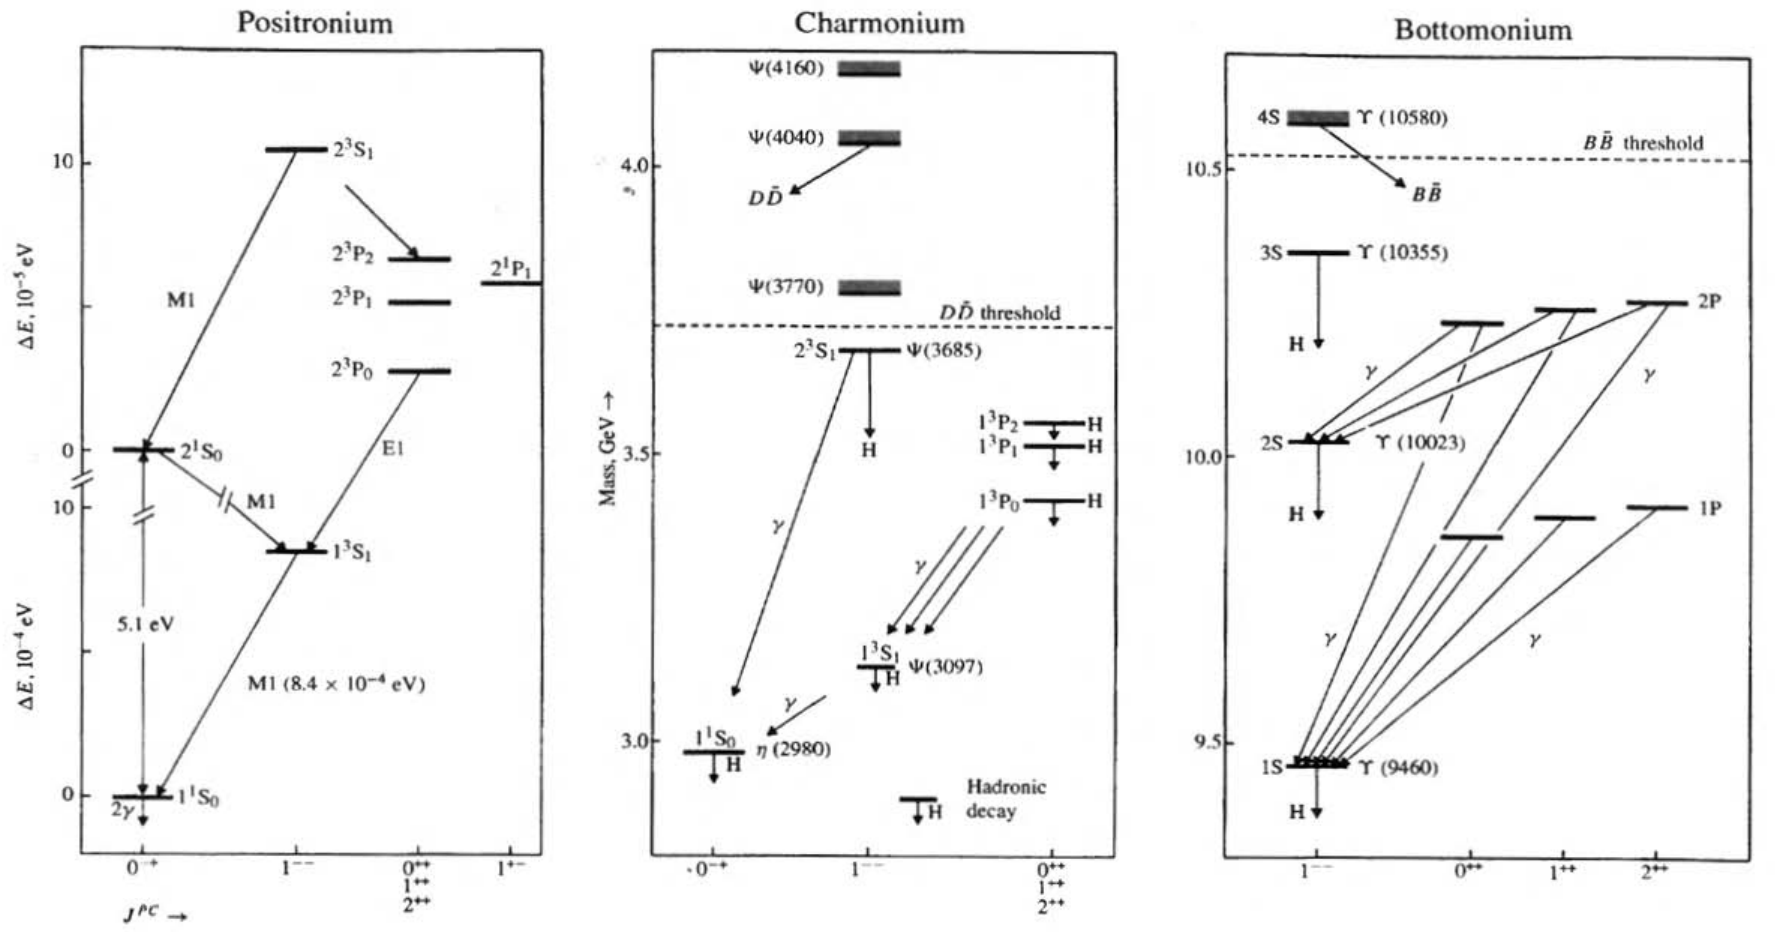
\includegraphics[width=1\linewidth]{Imagenes/NivelesEnergiaEECCBB.png}
    \caption{Niveles de energía del positrionio, charmonio ($c\bar{c}$) y bottomonio ($b\bar{b}$). }
    \label{fig:espectros eeccbb}
\end{figure}
La energía y la masa del charmonio $(c\bar{c})$ vienen dadas por 
$$E_n^{(c\bar{c})}=-\frac{1}{2}\mu c^2 \frac{\alpha_s^2}{n^2} \ \text{con} \ \mu=\frac{m_c}{2} \Rightarrow M_{c\bar{c}}=2mcc^2+E_n^{c\bar{c}}=2m_cc^2 \qty(1-\frac{\alpha_s^2}{8n^2})$$
Si comparamos con los datos experimentales y utilizamos la masa de la tabla \ref{tab: Particulas elementales} obtenemos que para el estado fundamental la masa debe ser $M_{c\bar{c}}\sim \unit[2.6]{MeV}$, que se desvía mucho de los datos experimentales.
\begin{table}[h]
\centering
\begin{tabular}{cc|c|c|}
\cline{3-4}
                                             &  & \textbf{$c\bar{c}$} & \textbf{$b\bar{b}$} \\ \hline
\multicolumn{1}{|c|}{\multirow{2}{*}{$n=1$}} & $^1S_0$   & 2984                & 9399                \\ \cline{2-4} 
\multicolumn{1}{|c|}{}                       & $^3S_1$   & 3097                & 9460                \\ \hline
\multicolumn{1}{|c|}{\multirow{6}{*}{$n=2$}} & $^3P_0$   & 3415                & 9860                \\ \cline{2-4} 
\multicolumn{1}{|c|}{}                       & $^3P_1$   & 3511                & 9892                \\ \cline{2-4} 
\multicolumn{1}{|c|}{}                       & $^3P_2$   & 3556                & 9913                \\ \cline{2-4} 
\multicolumn{1}{|c|}{}                       & $^1P_1$   & 3525                & 9899                \\ \cline{2-4} 
\multicolumn{1}{|c|}{}                       & $^1S_0$   & 3638                & 9999                \\ \cline{2-4} 
\multicolumn{1}{|c|}{}                       & $^3S_1$   & 3686                & 10023               \\ \hline
\multicolumn{1}{|c|}{$n=3$}                  & $^3S_1$   & 4040                & 10355               \\ \hline
\multicolumn{1}{|c|}{$n=4$}                  & $^3S_1$   & 4415                & 10580               \\ \hline
\end{tabular}
\caption{Datos experimentales de las masas de los estados de charmonio y bottomonio}
\label{tab: charmonio y bottomonio datos experimentales}
\end{table}

Debemos utilizar  $\alpha_s^2=1.623$ y la \textbf{masa constituyente} de los quarks $c/\bar{c}$, $m_cc^2=\unit[1942]{MeV}$, esta masa es análoga a la masa efectiva en física del estado sólido y representa la influencia de la interacción entre los quaks en el estado ligado.\\\\
Sabemos que el potencial de la interacción fuerte debe incluir un término de confinamiento ya que los quarks no existen libres en la naturaleza, ésto se comprueba al intentar separar los quarks que forman un mesón. Si los intentamos separar alcanzaremos energías que permitan crear una pareja quark-antiquark y se formarán más mesones. A este fenómeno se le conoce como \textbf{confinamiento} y nos sugiere que el potencial de la interacción fuerte debe tener un término adicional.
\\\\
Si intentamos ajustar este término con los potenciales más usuales, pozo infinito cuadrado, oscilador armónico, potencial lineal... El que reproduce mejor las medidas experimentales es el potencial lineal.
\begin{equation*}
    V_\mathrm{c}(x)=\left \{  \begin{aligned}
        &\Lambda^2 x \ \text{si} \ x\ge0 \\
        & 0 \ \text{si} \ x<0
    \end{aligned}\right.
\end{equation*}
Si resolvemos la ecuación de Schrödinger con dicho potencial, la solución es analítica y se conoce como funciones de Airy ($\mathrm{Ai}(x)$), así la ecuación de ondas será
\begin{equation*}
    \Psi_n(x)=N\qty(2m\hbar \Lambda^2)^{1/3} \mathrm{Ai}\qty(\qty(2m\hbar \Lambda^2)^{1/3}+\qty(x-\frac{E_n}{\Lambda^2})\frac{1}{\hbar})
\end{equation*}
Si imponemos que la función de onda ha de anularse en el orígen, es decir $\Psi_n(0)=0$, encontramos que $$E_n=\frac{\Lambda^2\hbar}{\qty(2m\hbar \Lambda^2)^{1/3}}(-\xi_n)$$ Donde $\xi_n$ son los ceros de las funciones de Airy.
\\\\
Es decir, que el potencial de la interacción fuerte a distancias cortas tiene un comportamiento del tipo coulombiano mientras que a largas distancias entra el juego el confinamiento y se comporta como un potencial lineal, al potencial que se comporta de esta manera se le conoce como \textbf{potencial de Cornell}
\begin{equation}
    V(r)=-\frac{k}{r}+\frac{r}{a^2}
\end{equation}
Este potencial no tiene solución analítica pero si introducimos la interacción spin-spin en teoría de perturbaciones reproducimos el espectro de energía de los mesones pesados de manera bastante precisa\footnote{Se puede completar más el espectro añadiendo términos de aniquilación.}. 

\section{Propiedades fundamentales de la interacción débil}
La interacción débil tiene un problema fundamental y es que \textbf{no} forma estados ligados. Por lo tanto debemos estudiarla a partir de reacciones.\\\\ Sólo se da en aquellos casos en los que las interacciones fuerte y electromagnética estén prohibidas. En consecuencia los procesos débiles tienen \textbf{vidas medias muy largas}, generando un espectro muy amplio ya que tenemos ejemplos como el neutrón con $\tau_n \sim \unit[10^3]{s}$ y el pión con $\tau_\pi \sim \unit[10^{-8}]{s}$ debido a que la diferencia de energías entre el estado final e inicial es muy pequeña (explicación en la sección \ref{sec: particulas virtuales}).
\newpage
\noindent
\begin{minipage}{0.5\linewidth}
    La interacción débil conserva:
\begin{itemize}
    \item Momento angular, $J$ y carga $Q$.
    \item Números leptónicos de cada familia, $L_i$.
    \item Número bariónico, $B$.
\end{itemize}
\end{minipage}
\hfill
\begin{minipage}{0.4\linewidth}
    La interacción débil no conserva:
    \begin{itemize}
        \item Paridad y $C-$paridad.
        \item Isospín y número de quarks.
        \item Sabor.
    \end{itemize}
\end{minipage}\\\\

Y viene mediada por 3 bosones gauge: $W^\pm, Z^0$. Hasta 1973, se entendían todos los procesos sólo con $W^\pm$ pero el Modelo Standar exigía la existencia del $Z^0$ que se descubrió a finales de los 70. Así podemos clasificar los procesos débiles en \textbf{corrientes cargadas}, mediadas por $W^\pm$; y \textbf{correntes neutras}, mediadas por $Z^0$.\\\\
Otra clasificación que podemos hacer es en función de las partículas que participan en las reacciones y que son
\begin{itemize}
    \item \textbf{Leptónicos}: Si \textbf{todas las partículas} son leptones. Por ejemplo: $\mu^- \longrightarrow e^- +\nu_\mu + \overline{\nu}_e$.
    \item \textbf{Semileptónicos}: Si involucra hadrones y leptones. Por ejemplo: $n \longrightarrow p+ e^-  + \overline{\nu}_e$
    \item \textbf{Hadrónicos}: Si \textbf{todas las partículas} son hadrones. Por ejemplo: $\Lambda \longrightarrow p +\pi^-$
\end{itemize}
\subsection{Corrientes cargadas. Procesos Leptónicos}
\noindent
\begin{minipage}{0.6\textwidth}
    En los procesos leptónicos el bosón débil se ``lleva'' la carga del leptón cargado, transformándolo en su correspondiente neutrino, y se la transfiere a un leptón más ligero, generando además el antineutrino correspondiente.\\\\
    Cada vértice del diagrama \ref{fig: desintegracion muon} es leptónico, por lo que tienen la misma carga $g_W$. Por lo tanto la probabilidad que tiene de darse este proceso es $P\sim \abs{\alpha_W}^2$ con $\alpha_W=\dfrac{\alpha}{m_W}$ y $\alpha \sim g^2$.
\end{minipage}
\hfill
\begin{minipage}{0.35\textwidth}
    \centering
    \includegraphics[width=0.8\textwidth]{Diagramas Tema 2/DesintegracionMuonII.pdf}
    \captionof{figure}{Desintegración débil del muón.}
    \label{fig: desintegracion muon}
\end{minipage}
\subsection{Corrientes cargadas. Procesos semileptónicos}
En estos procesos encontramos tanto quarks como leptones. Si intentamos medir cómo se acopla el mesón $W^-$ a los quarks tenemos un problema, pues los quarks tienen color y no seríamos capaces de ver la reacción fundamental. Para estudiar estos procesos se hicieron dos hipótesis
\newpage
\subsubsection{Simetría quark-leptón}
\noindent
\begin{minipage}{0.6\textwidth}
    Los leptones y los quarks los tenemos agrupados en 3 familias. Puesto que todas las partículas participan en la interacción débil, se postuló que los quarks de la 1ª familia $(u,d)$ participan de la misma manera que los leptones de la 1ª familia $(e^-,\nu_e)$.\\\\
Cuando se introdujo esta simetría, no se conocía el quark $c$. Pero ahora podemos generalizarlo también a la 2ª familia, así
\begin{equation}
    \mqty(u\\d) \Leftrightarrow \mqty(e^-\\\nu_e), \quad \mqty(c\\s) \Leftrightarrow \mqty(\mu^-\\\nu_\mu) 
\end{equation}
En la sección \ref{sec: universalidad de la interaccion debil}, demostramos que las diferentes familias de leptones participaban de igual manera en la interacción débil. Por lo tanto si asociamos $g_W$ a $W^\pm$, como ya hicimos en los procesos leptónicos, esa $g_W$ será la misma para todos los leptones, lo que significa que $g_W=g_{ud}=g_{cs}$.
\end{minipage}
\hfill
\begin{minipage}{0.35\textwidth}
    \centering
    \includegraphics[width=\textwidth]{Diagramas Tema 2/DiagramadeQuarksBeta-.pdf}
    \captionof{figure}{Diagrama de Feynmann de la desintegración $\beta^-$.} \label{fig: desintegracion beta}
    \vspace{1.5cm}
    \includegraphics[width=\textwidth]{Diagramas Tema 2/DesintegracionPion+.pdf}
    \captionof{figure}{Diagrama de Feynmann de la desintegración del $\pi^-$.} \label{fig: desintegracion pion}
\end{minipage}\\\\

\noindent Por ello, como el $W^\pm $ mezclaba leptones de la misma familia, también lo hará con quarks de la misma familia. Fue así como se pudo entender los procesos \ref{fig: desintegracion beta} y \ref{fig: desintegracion pion}.
\subsubsection{Mezcla de quarks. Postulado de Cabibbo}
Aunque se entendían muchos de los procesos debido a la simetría quark-leptón, había un proceso que no se entendía ya que mezcla distintas familias de quarks.
$$K^-(s\bar{u})\longrightarrow \mu^-+\bar{\nu}_\mu$$

Cabibbo definió un estado $d^\prime$ que es combinación del quark $d$ y $s$. Así la 1ª familia de quarks está formada por $\mqty(u\\d^\prime)$. Este nuevo estado se define como 
\begin{equation}
d^\prime=d\cos(\theta_\mathrm{C})+s\sin(\theta_\mathrm{C})
\label{eq: estado mezcla ds}
\end{equation}
Así podemos tener vértices que mezclan $(u,d)$ y $(u,s)$ (Figura \ref{fig:vertices UD}), modificando así el valor de las constantes de interacción de esos vértices.
\begin{equation}
    \begin{aligned}
        &g_{ud}=g_W \cos{(\theta_\mathrm{C})}\\
        &g_{us}=g_W \sin{(\theta_\mathrm{C})}
    \end{aligned}
    \label{eq: constantes mezcla}
\end{equation}
\begin{figure}[h]
    \centering
    \includegraphics[width=0.5\linewidth]{Diagramas Tema 2/VerticesUD.pdf}
    \caption{Vértice ($ud^\prime W$) y su interpretación como suma de vértices ($udW$) y ($usW$). El vértice $(usW)$ está suprimido por el ángulo de Cabibbo.}
    \label{fig:vertices UD}
\end{figure}
Ahora bien, tenemos que tener en cuenta que el ángulo de Cabibbo $(\theta_\mathrm{C})$, debe ser pequeño para no modificar lo que conocemos sobre la desintegración del pión y que esté suprimido para el kaón
\newpage
Tras la propuesta de la existencia del quark $c$ por parte de Glashow, Iliopoulos y Maiani (GIM) en 1970, se modificó la teoría de Gell-Mann de la existencia de un doblete y un singlete a dos dobletes y en analogía al quark $d$, se introdujo un estado $s^\prime$ ortogonal al estado $d^\prime$
\begin{equation}
    s^\prime=-d\sin(\theta_\mathrm{C})+s\cos(\theta_\mathrm{C}) 
    \label{eq: estado mezcla sd}
\end{equation}

La introducción del quark encantado permite introducir una matriz para pasar de los quarks físicos a los quarks descritos por la teoría débil a través de 
\begin{equation}
   Q= \mqty(-\sin(\theta_\mathrm{C}) & \cos(\theta_\mathrm{C})\\
    \cos(\theta_\mathrm{C}) &\sin(\theta_\mathrm{C}))
    \label{eq: matriz ckm}
\end{equation}
que se conoce como matriz de intercambio de quarks. Además introduce un nuevo número cuántico \textbf{el encanto}.
Así las constante de interacción \ref{eq: constantes mezcla} serán
\begin{equation}
    \begin{aligned}
        &g_{ud}=g_{cs}=g_W \cos{(\theta_\mathrm{C})}\\
        &g_{us}=-g_{cd}=g_W \sin{(\theta_\mathrm{C})}
    \end{aligned}
    \label{eq: constantes mezcla total}
\end{equation}
Y a los vértices descritos en la figura \ref{fig:vertices UD} tenemos que añadir también los producidos por la desintegración del $c\xrightarrow[]{} s^\prime+W^+$
\begin{figure}[h]
    \centering
    \includegraphics[width=0.5\linewidth]{Diagramas Tema 2/VerticesDS.pdf}
    \caption{Vértice ($cs^\prime W$) y su interpretación como suma de vértices ($cdW$) y ($csW$). El vértice $(cdW)$ está suprimido por el ángulo de Cabibbo debido a la expresión \ref{eq: estado mezcla sd}.}
    \label{fig:vertices DS}
\end{figure}

Ahora queremos determinar el ángulo de Cabibbo, para ello vamos a comparar la desintegración del kaón y la desintegración del pión y la del neutrón y el muón.
\begin{equation}
  \left.  \begin{aligned}
        &\frac{\Gamma\qty(K^-\xrightarrow{}\mu^-+\bar{\nu}_\mu)}{\Gamma\qty(\pi^-\xrightarrow{}\mu^-+\bar{\nu}_\mu)} \sim \frac{g_{us}^2}{g_{ud}^2} \sim \tan^2(\theta_\mathrm{C})\\\\
        &\frac{\Gamma\qty(n\xrightarrow{}p+e^-+\bar{\nu}_e)}{\Gamma\qty(\mu^-\xrightarrow{}e^-+\bar{\nu}_e+{\nu}_\mu)} \sim \frac{g_{ud}^2}{g_{W}^2} \sim \cos^2(\theta_\mathrm{C})
    \end{aligned} \right \} \Rightarrow \theta_\mathrm{C}=13^{\degree}
\end{equation}

\noindent De la comparación de estas dos reacciones tenemos que $\dfrac{g_{us}^2}{g_{ud}^2}=\dfrac{g_{cd}^2}{g_{cs}^2}=\tan^2(\theta_{C})$, con lo que todos los procesos débiles que contengan un quark $c$ en el estado final estarán favorecidos a tener un quark $s$ en el estado final. Esto hace que todo aquello que vaya medido por $g_{us}$ y $g_{cd}$ son procesos suprimidos por Cabibbo; y los medidos por $g_{ud}$ y $g_{cs}$ están favorecidos. \\\\
Así tenemos que los decaimientos del quark $c$ en quarks ligeros por el ángulo de Cabibbo son
\begin{equation}
    \begin{aligned}
        &c\longrightarrow s+l^++\nu_l \quad \text{con} \quad l=e,\mu\\
        & c\longrightarrow s+u+\bar{d}
    \end{aligned}
    \label{eq: Decaimientos favorecidos c}
\end{equation}

\subsubsection{Reglas de selección}
De la teoría de Cabibbo podemos extraer reglas de selección para no tener necesidad de dibujar el diagrama de quarks.\\\\
Para estudiar la regla de selección en procesos semileptónicos estudiemos los siguientes procesos
\begin{equation*}
    \begin{aligned}
        &\Sigma^- \longrightarrow n+e^-+\bar{\nu}_e \\
        &\Sigma^+ \longrightarrow n+e^++\nu_e
    \end{aligned}
\end{equation*}
Si comparamos los espacios fásicos son exactamente iguales por lo que podríamos suponer que $R_\mathrm{th}=\dfrac{\Gamma\qty(\Sigma^+ \longrightarrow n+e^++\nu_e)}{\Gamma\qty(\Sigma^- \longrightarrow n+e^-+\bar{\nu}_e)}\simeq 1$ pero experimentalmente hemos sabemos que $R_\mathrm{exp}<5\cdot 10^{-3}$. \\\\
Debemos tener en cuenta supresión de Cabibbo, para ello estudiamos la parte hadrónica de ambos procesos
\begin{equation*}
    \begin{aligned}
        &\mathrm{Proceso} \ \Sigma^- : \quad dds \longrightarrow ddu \\
        &\mathrm{Proceso} \ \Sigma^+:  \quad uus \longrightarrow udd
    \end{aligned}
\end{equation*}

Por lo tanto en el proceso $\Sigma^-$ tenemos que cambiar un quark $s$ por un quark $u$ mientras que en el proceso $\Sigma^+$ tenemos que cambiar dos quarks $u\leftrightarrow d$ y $s \leftrightarrow d$, es decir, tenemos dos cambios de sabor (dos emisiones de un bosón $W$), lo cual la probabilidad de este proceso es despreciable ($P\sim \abs{\alpha_W}^4$).\\\\
Vamos a analizar procesos que sólo\footnote{Nos centramos en la parte hadrónica, a los leptones no afecta a este análisis.} incluyan quarks ligeros y extraños, en estos procesos tenemos dos casos
\begin{itemize}
    \item \textbf{No aparecen quarks extraños}: El intercambio $u\leftrightarrow d$ por lo tanto $\Delta Q=\pm 1$ y $\Delta s=0$.
    \item \textbf{Presencia de quarks extraños}: En estos procesos tenemos la siguiente transformación $$\left \{ \begin{aligned}
        &u\xrightarrow{} s+W^+ \Rightarrow \Delta s =-1=\Delta Q\\
        &s\xrightarrow{} u+W^- \Rightarrow \Delta s =+1=\Delta Q
    \end{aligned} \right.$$
    Por lo que la regla de selección es $\Delta s=\Delta Q=\pm 1$. 
\end{itemize}

Esto garantiza procesos a primer orden, que para el proceso $\Sigma^-, \Delta Q=\Delta s=1$ mientras que para el proceso $\Sigma^+, \Delta Q=-1, \Delta s=+1$ por lo que está \textbf{suprimido} a primer orden.\\\\
Ahora vamos a calcular las reglas de selección para procesos que incluyen encanto. Para ello utilizamos los decaimientos \ref{eq: Decaimientos favorecidos c}, para ello estudiamos las desintegraciones del mesón $D^+(c\bar{d})$:
\begin{equation*}
    \begin{aligned}
        &(1): \quad D^+ \longrightarrow K^-+\pi^++e^++\nu_e \\
        &(2): \quad D^+ \longrightarrow \pi^-+\pi^++e^++\nu_e
    \end{aligned}
\end{equation*}
Como hicimos para los procesos con extrañeza analizamos la parte hadrónica de ambos procesos
\begin{equation*}
    \begin{aligned}
        &\text{Proceso} \ (1): c\bar{d}\xrightarrow[]{} \bar{u}s+u\bar{d}\\
        &\text{Proceso} \ (2):c\bar{d}\xrightarrow[]{} \bar{u}d+u\bar{d}
    \end{aligned}
\end{equation*}

En el proceso (1) los incrementos de sabor y carga son $\Delta c=-1,\Delta s=-1, \Delta Q=-1$. En el proceso (2) los incrementos de sabor y carga son $\Delta c=-1,\Delta s=0, \Delta Q=-1$. Ahora si tenemos en cuenta que los decaimientos favorecidos \ref{eq: Decaimientos favorecidos c} son los que tienen incremento de extrañeza, por lo tanto $\Delta c=-1, \Delta s=-1, \Delta Q=-1,0$ \footnote{Quitamos la contribución de $\Delta Q=0$ ya que en corrientes neutras los cambios de sabor están suprimidos (página siguiente).}. Por lo tanto $\boxed{\Delta s=\Delta c=\Delta Q=\pm 1}$.
\subsection{Corrientes cargadas. Procesos hadrónicos}
Estos procesos están descritos por simetría Quark-Leptón + Mezcla de Quarks. Estos procesos sólo tienen hadrones en ambos lados de la reacción como vimos en la figura \ref{fig: diagrama de quarks delta ++ posible}.
\subsubsection{Reglas de selección. Incremento de extrañeza}
En estos procesos necesariamente la carga se tiene que conservar, por lo tanto $\Delta Q=0$ y sólo tenemos cambios en la extrañeza $\Delta s=0,\pm1$.\\\\
Vamos a suponer que el barión cascada $\Xi^- (ssd)$ se puede desintegrar por los siguientes canales:
\begin{equation*}
    \begin{aligned}
        &\quad \Xi^- \longrightarrow \Lambda^0+\pi^- \ \Delta Q=0 \ \Delta s=+1 \\
        &\quad \Xi^- \longrightarrow n+\pi^- \ \Delta Q=0 \ \Delta s=+2
    \end{aligned}
\end{equation*}
En la naturaleza sólo se observa el primer proceso, pues el segundo necesita de al menos dos bosones $W$. Análogamente para la partícula $\Omega^-$ tenemos la siguiente cadena
$$\Omega^-\xrightarrow[]{} \textcolor{red}{\Xi^0}+\pi^- \xrightarrow[]{} \textcolor{red}{\Lambda^0}+\pi^0 \xrightarrow[]{} \textcolor{red}{p+\pi^-}$$

\noindent Cada una de los diferentes pasos tienen un cambio de extrañeza $\Delta s=+1$.
\subsubsection{Reglas de selección. Incremento de isospín}

Como ya sabemos el isospín no es una simetría de la interacción débil, dentro de los procesos hadrónicos hay observaciones fenomenológicas acerca de la preferencia de isospín en la naturaleza. Esta violación de isospín la naturaleza va a hacerla en la menor cantidad posible, por lo que la regla de selección es 
\begin{equation}
    \boxed{\Delta s=1, \ \abs{\Delta I}=\frac{1}{2}}
\end{equation}

\noindent Esto se entiende debido a que el cambio $[s (I=0)\leftrightarrow u,d(I=\nicefrac{1}{2})]$.
%Aqui no se si hacer el ejemplo con el teorema de Wigner-Eckart y explicarlo con los apuntes de Eliecer.

\subsection{Corrientes neutras}
Estas corrientes vienen mediadas por el intercambio de bosones $Z^0$. Como necesariamente se tienen que conservar los números leptónicos y la carga, sólo tenemos dos vías por las que se pueden dar las corrientes neutras
\begin{figure}[h]
    \centering
    \includegraphics[width=0.5\linewidth]{Diagramas Tema 2/VerticesNeutros.pdf}
    \caption{Vertices neutros.}
    \label{fig:Vertices neutros}
\end{figure}

Para que en las corrientes neutras podamos tener hadrones necesitamos introducir de nuevo \textbf{simetría quark-laptón + mezcla de quarks}. \\\\ Podemos tener 6 vértices neutros (quarks de la 3ª familia) no suprimidos: $$\nu_e\nu_e Z^0 \quad \nu_\mu\nu_\mu Z^0 \quad e^-e^- Z^0 \quad \mu^-\mu^- Z^0 \quad uu Z^0 \quad d^\prime d^\prime Z^0$$

Fijémonos que estos vértices no tienen intercambio de sabor ya que son los suprimidos, demostrémolos:
\begin{equation*}
    \begin{aligned}
    & d^\prime d^\prime Z^0=ddZ^0 \cos^2\theta_\mathrm{C}+ssZ^0 \sin^2\theta_\mathrm{C} +(dsZ^0+sdZ^0\cos\theta_\mathrm{C})\sin\theta_\mathrm{C}\cos\theta_\mathrm{C}\\
    & s^\prime s^\prime Z^0=ddZ^0 \cos^2\theta_\mathrm{C}+ssZ^0 \sin^2\theta_\mathrm{C} -(dsZ^0+sdZ^0\cos\theta_\mathrm{C})\sin\theta_\mathrm{C}\cos\theta_\mathrm{C}
    \end{aligned}
\end{equation*}

\noindent Que si sumamos ambos vértices vemos que los intercambios de sabor de quarks se suprimen.\\\\
Por lo tanto, los vértices neutros de quarks conservan extrañeza y encanto, al contrario que los vértices de las corrientes cargadas.
Esto se puede comprobar experimentalmente a partir de los decaimientos de los kaones.
\begin{equation*}
    \begin{aligned}
        &K^+\longrightarrow \pi^0 +\mu^++\nu_\mu \quad BR_i=3.35 \cdot 10^{-2} \quad \text{Corriente cargada}\\
        &K^+\longrightarrow \pi^+ +\nu_l+\bar{\nu}_l \ \quad BR_i<1.14\cdot 10^{-10} \quad \text{Corriente neutra}
    \end{aligned}
\end{equation*}

\noindent Si estudiamos las anchuras de desintegración de todos estos procesos $$R_\mathrm{exp}=\frac{\sum_l \Gamma\qty(K^+\xrightarrow[]{} \pi^++\nu_l+\bar{\nu}_l)}{\Gamma\qty(K^+\xrightarrow[]{} \pi^0+\mu^++\nu_\mu )}<10^{-7}$$

Por lo que el proceso neutro está suprimido debido al cambio de extrañeza.
\subsection{Violación de paridad}
La no universalidad de la paridad en los procesos físicos fue una cuestión que trajo muchos dolores de cabeza hasta 1956. En los años 50 había un problema en la física de partículas llamado ``puzzle de la partícula $\tau-\theta\,$'' donde se conocía $\tau \xrightarrow[]{} 2\pi$ y $\theta \xrightarrow[]{} 3\pi$. Hasta que la $\theta$ se midió un modo de desintegración $\theta\xrightarrow[]{} \pi^++\pi^0$. Como los piones tienen $J^P=0^-$, por lo que si imponemos conservación de momento angular tenemos ${J}_\theta={L}_{\pi \pi}$ si imponemos conservación de paridad, el acoplo de momentos angulares debe ser en onda S para paridad + y en onda P para paridad -, por lo que obtenemos la siguiente serie 
$J^P_\theta=0^+,1^-+2^+...$ \\\\
En el caso de la $\tau$ se había medido un modo cargado $\tau^+\xrightarrow[]{} 2\pi^++ \pi^-$ en el que $J^P_\tau=0^-$, por lo que los momentos angulares relativos debían ser iguales.\\\\
Experimentalmente se demostró que estas partícula tenían spin nulo y la misma masa por lo que necesariamente debían ser la \textbf{misma partícula}. Esto supone un problema ya que debemos tener una paridad distinta para una misma partícula.
\subsubsection{Hipótesis de Lee y Yang}

Lee y Yang supusieron que la paridad no se conservaba estrictamente, para decir que $\theta$ y $\tau$ son dos modos de decaimiento de la misma partícula. Esto se puede suponer como una evidencia de que la paridad no se conserva en la interacción débil.
\\\\
Esto trae consigo otro problema, no se conserva con la C-paridad. El hecho de que las partículas y las antipartículas tuvieran la misma media se demostraba como invarianza bajo transformaciones de C-paridad. Aunque esto también se puede demostrar suponiendo invarianza bajo \textbf{transformaciones de Lorentz} como vimos con la ecuación\ref{eq: Ecuacion de Klein-Gordon}.\\\\
En 1956 Madame Wu demostró que la hipótesis de Lee y Yang era correcta, para ello se midió la interacción débil de los núcleos de cobalto-60, que se desintegra por $\beta^-$. Através de $^{60}\mathrm{Co}\xrightarrow[]{}^{60}\mathrm{Ni}+e^-+\bar{\nu}_e$. En los núcleos es fácil determinar el spin y la paridad, por lo que se planteó medir la distribución angular de los electrones emitidos y así determinando si existe una dirección privilegiada para estos electrones.\\\\
Se podían dar dos situaciones:
\begin{itemize}
    \item Si el proceso fuese invariante bajo paridad, la probabilidad debería ser la misma en las direcciones perpendicular y antiperpendicular al campo magnético \footnotemark. 
    \item Si el proceso no fuese invariante bajo paridad, si que existe una dirección privilegiada
\end{itemize}
\footnotetext{Para determinar el spin necesitamos el campo magnético como en el experimento de Stern-Gerlach}

Lo que se observó fue que se emitían más electrones en la dirección contraria al campo por lo que \textbf{no se conservaba} la paridad.